\documentclass{elsart}
\usepackage[dvips]{color,graphics}
\usepackage[pdftex]{graphicx}
\usepackage{lineno}
\linenumbers
%
% macro definitions

%\setcounter{tocdepth}{1} % Show sections
%\setcounter{secnumdepth}{0}


%\setcounter{bottomnumber} {1}
%
%\pagenumbering{arabic}
%
\begin{document}

% -------------------------------------------------
%  title page
% -------------------------------------------------
\begin{frontmatter}
  
\title{The CLAS12 Drift Chamber System}


\author[jlab]{M.D. Mestayer},
\author[hampton]{K. Adhikari},
\author[odu]{R.P. Bennett},
\author[odu]{S. Bueltmann},
\author[msu]{T. Chetry},
\author[jlab]{S.B. Christo},
\author[jlab]{M. Cook IV},
\author[jlab]{R.C. Cuevas},
\author[odu]{G.E. Dodge},
\author[isu]{T.A. Forest},
\author[jlab]{G. Jacobs},
\author[odu]{T. Hartlove},
\author[wm]{T.B. Hayward},
\author[ucriverside]{L. Kabir},
\author[odu]{S.E. Kuhn},
\author[isu]{D. McNulty},
\author[jlab]{W.M. Taylor},
\author[odu]{L.B. Weinstein},
\author[jlab]{V. Ziegler}
\address[jlab]{Thomas Jefferson National Accelerator Facility, Newport News, VA 23606, USA}
\address[odu]{Old Dominion University, Norfolk, VA 23529}
\address[isu]{Idaho State University, Pocatello, ID 83209}
\address[msu]{Mississippi State University, Mississippi State, MS 39762}
\address[wm]{The College of William and Mary, Williamsburg VA 23185}
\address[hampton]{Hampton University, Hampton VA 23669}
\address[ucriverside]{University of California, Riverside, Riverside CA 92521}

\date{\today}


% -------------------------------------------------
%abstract
% -------------------------------------------------

\begin{abstract}

Experimental Hall B at Jefferson Laboratory houses the CEBAF Large
Acceptance Spectrometer, the magnetic field of which is produced by a
superconducting toroid.  The six coils of this toroid divide the detector
azimuthally into six sectors.  Each sector contains three multi-layer 
drift chambers for reconstrucing the trajectories of charged particles
emanating from a fixed target.  Each of the 18 chambers has a total of 1344
individually instrumented drift cells.  The wires are arranged in planar
layers, and each chamber has two `superlayers' of six layers each. 
The six-layer structure allows for redundancy in track segment finding
and facilitates good tracking efficiency even in the presence of some
individual wire inefficiency.  The design, construction, operation and
calibration methods are described and estimates of efficiency and resolution
are presented from in-beam measurements.

\end{abstract}






\end{frontmatter}
%\tableofcontents
%\listoffigures
%\listoftables


\section{Forward Tracking System}
\label{overview}

The CLAS12 forward detector is constructed around a toroidal magnet consisting of six 
iron-free superconducting coils.  The particle detection system consists of drift 
chambers to determine charged-particle trajectories, {\v C}erenkov detectors 
for electron/pion separation, scintillation counters for flight-time 
measurements, and calorimeters to identify electrons and high-energy neutral 
particles.  An overview of the CLAS12 subsystems and geometry may be found in the 
CLAS12 Overview paper ~\cite{clas12-overview} in this volume.  A schematic view of the 
torus magnet with drift chambers
attached is shown in Fig.~\ref{chambers-and-torus}.   The drift chambers are 
triangular boxes attached to the magnet cryostat by ``rod and ball and socket'' sets.  
This assembly of magnet and chambers is referred to as the ``forward tracker''. 

The forward tracker can detect charged particles emerging from the target with
momenta greater than 200~MeV/c over a polar angular range from roughly 5$^{\circ}$ to 
40$^{\circ}$.  Because the coils of the torus magnet represent a ``dead area''
in which we cannot detect charged particles, we designed the chamber endplates
and attached electronics to be as thin as possible.  The resulting azimuthal
coverage varied from 50\% of 2$\pi$ at 5$^{\circ}$ to 80\% of 2$\pi$ at 40$^{\circ}$.


%%%%%%%%%%%%%%%%%%%%%% Figure : CLAS 3D Picture %%%%%%%%%%%%%%%%%%%%%%%%%%%%%%%
\begin{figure}[htbp]
\vspace{10cm}
\begin{picture}(50,50)
\put(-10,10)
{\hbox{\includegraphics[width=0.5\textwidth,natwidth=610,natheight=642]{img/chambers-and-torus.png}}}
\end{picture}
\caption{\small{A sketch of the torus magnet with drift chambers attached.
Note that cable runs and gas lines have been removed for clarity.  The largest
(R3) chambers are approximately equilateral triangular solids with 4 m long sides
and 0.8 m depth.}}
\label{chambers-and-torus}
\end{figure}
%%%%%%%%%%%%%%%%%%%%%%%%%%%%%%%%%%%%%%%%%%%%%%%%%%%%%%%%%%%%%%%%%%%%%%%%%%%






















































% -------------------------------------------------
% physics goals -> tech. specs. -> conceptual design
% -------------------------------------------------

\section{Drift Chamber System Conceptual Design}

When the CLAS detector was upgraded to the CLAS12 detector, the
drift chambers were re-designed.  We kept many of the design concepts
of the original CLAS chambers, but made improvements in a number
of areas.

\subsection{Physics Requirements for {\tt CLAS12} Forward Tracking}

There are several broad areas of physics research that drive 
the design of the forward tracking system: 
spectroscopic studies of excited baryons, investigations of 
the influence of nuclear matter on propagating quarks, studies of polarized 
and unpolarized quark distributions, and a comprehensive measurement of 
generalized parton distributions (GPDs). 

The cross sections for these processes are small, necessitating high-luminosity 
experiments.  A variety of simulated experiments rely on luminosities of 
10$^{35}$~cm$^{-2}$s$^{-1}$ to achieve the desired statistical accuracy in 
runs of a few months duration.  This is an order of magnitude increase
in beam flux compared to the previous CLAS detector.  

The new kinematic range available to the CLAS12 experiment is
characterized not only by smaller cross sections, but also by more outgoing 
particles per event, with those particles being emitted with higher values 
of momentum and at smaller laboratory angles.  
A final state of a few high-momentum, forward-going particles (the electron as well as one 
or more mesons), combined with a moderate-momentum baryon emitted at large 
angles, is the typical event type that determines the specifications of the 
tracking system. 

The forward detector must provide tracking for laboratory angles between 5$^\circ$ 
and 40$^\circ$ in order to cover as much of 
the hadronic center-of-mass region as possible.  

We require very good momentum 
and angular resolution for the scattered electron in order to determine the 
virtual photon flux factor, $\Gamma_v$, to an accuracy of a few percent.
Equally important, we must have good momentum resolution on the scattered
electron (with momentum up to 10 GeV/c) to be able to identify particles
by missing mass, an important technique in exclusive reaction studies.
Our design specification on the fractional momentum resolution was set to
$dp/p = 0.3\%$ for electrons emitted at small angles ($~ 7^{circ}$) and high
momentum ($~ 10 GeV/c$) to insure our ability to efficiently identify
particles by missing mass.  Angular resolutions of 1~mrad are required for the electron 
in order to know the virtual photon flux factor, and hence, the cross section, 
to a few percent. 

Table~\ref{fwd-dc-physics-specifications} lists the physics goals for the CLAS12 program
main and the resulting design specifications that will allow us to achieve these goals.

%%%%%%%%%%%%%%%%%%%%%%%%%%%%%%%%%%%%%%%%%%%%%%%%%%%%%%%%%%%%%%%%%%%%%%%%%
\small{
\begin{table}[ht]
\begin{center}
\begin{tabular}{||c|c|c||} \hline \hline
   {\bf Goal}         & {\bf Physics Specification} & {\bf Design Specification}\\ \hline
Measure $\Gamma_v$  & $d \theta < 1mrad$   & planar chambers \\ 
accurately  & $dp/p < 1\% $ & identical cells (each superlayer)  \\ \hline
Select an exclusive  &    & $250~\mu$m  accuracy \\ 
reaction; e.g. only one    & $dp/p < .3\% at 10 GeV/c$ &    $+/- 6^\circ$ stereo angle  \\ 
missing pion       & & chamber alignment $<100\mu$ \\ \hline
Small       & L = $10^{35}$~cm$^{-2}$s$^{-1}$  & six 6-layer superlayers \\ 
cross sections  & high efficiency & 95\% layer efficiency \\ \hline
good acceptance   & $\delta\phi = 50\%$ at $5^\circ$ & thin endplates\\ \hline
\end{tabular}
\caption{\small{\bf Physics goals and the resulting physics and design specifications.}}
\label{fwd-dc-physics-specifications}
\end{center}
\end{table}
}
%%%%%%%%%%%%%%%%%%%%%%%%%%%%%%%%%%%%%%%%%%%%%%%%%%%%%%%%%%%%%%%%%%%%%%%%%

\subsection{Drift Chamber Conceptual Design and Specifications}

The overall tracking requirements (0.3\% fractional momentum resolution 
at 10~GeV and efficient tracking at a luminosity of 
10$^{35}$~cm$^{-2}$s$^{-1}$) are the main drivers for the drift chamber design.  

Because the previous {\tt CLAS} drift chamber system~\cite{dcnim} operated 
successfully for 8~years, we re-used many of the design concepts and 
most of the utility infrastructure.  For example, we re-used some
parts of the gas mixing and handling system, and also the high-voltage 
and low-voltage systems and many of the high voltage and signal cables. 
Refer to our 
article on the previous {\tt CLAS} detector~\cite{clasnim} and our article 
on the previous drift chambers themselves~\cite{dcnim} for details of the 
previous detector and chambers.  

We kept the same chamber layout as ub {\tt CLAS}:
the forward tracking system consists of three regions divided into six
sectors as shown in Fig.~\ref{chambers-and-torus}; located just before, inside, 
and just outside the torus field volume, and referred to as Regions~1, 2, 
and 3, respectively.  
Each chamber has its wires arranged in two superlayers (SL) of
six layers each, with the wires in the two superlayers strung with 
$\pm$6$^\circ$ stereo angles, respectively.  The cell structure is 
hexagonal, that is, each sense wire is surrounded by six field wires.  This 
arrangement offers good 
resolution with very good pattern recognition properties.  

The major difference compared to the previous design is that the 
cells cover a smaller solid angle than those in the previous {\tt CLAS} 
chambers, allowing efficient tracking at higher luminosities because the 
accidental occupancy from particles not associated with the event is smaller.  

\subsection{Design Features}

Table~\ref{fwd-dc-design-parms} lists the main design parameters for each 
region of the {\tt CLAS12} drift chambers.  For the purposes of simulating 
track resolutions, we assumed that the position resolution of the individual 
drift cells would be 250~$\mu$m.  

%%%%%%%%%%%%%%%%%%%%%%%%%%%%%%%%%%%%%%%%%%%%%%%%%%%%%%%%%%%%%%%%%%%%%%%%%
\small{
\begin{table}[ht]
\begin{center}
\begin{tabular}{||c|c|c|c||} \hline \hline
            &{\bf Region 1}&{\bf Region 2}&{\bf Region 3}\\ \hline
Distance from target & 2.3 m    & 3.5 m        & 4.9 m    \\ \hline
Num. of superlayers  & 2        & 2            & 2        \\ \hline
Layers/superlayer    & 6        & 6            & 6        \\ \hline
Wires/layer          & 112      & 112          & 112      \\ \hline
Cell radius (each SL) & 0.78, 0.81 cm  & 1.14. 1.32 cm      & 1.87, 1.96 cm  \\ \hline
Active time window   & 150 ns   & 325 - 1000 ns & 750 ns   \\ \hline
\end{tabular}
\caption{\small{Design parameters for the {\tt CLAS12} drift chambers.}}
\label{fwd-dc-design-parms}
\end{center}
\end{table}
}
%%%%%%%%%%%%%%%%%%%%%%%%%%%%%%%%%%%%%%%%%%%%%%%%%%%%%%%%%%%%%%%%%%%%%%%%%

\subsubsection{Design Elements in Common with the Previous CLAS Chambers}
The CLAS12 drift chambers share some design characteristics with the
previous CLAS chambers:
\begin{itemize}
\item Wire Layout
\begin{itemize}
\item ``brick-wall'' wire layout resulting in individual hexagonally-shaped
drift cells
\item sense wire layers are grouped into two ``superlayers'' of 6 layers each
\item the ``endplates'' on the two sides of the chamber are tilted 
at approximately 60 deg. with respect to each other
\end{itemize}
\item Chamber Body Design
\begin{itemize}
\item to maximize the active volume of the chamber, the ``dead areas'', e.g.
the endplates and electronics boards are kept as thin as possible
\item because of the possibility of large eddy currents and resultant
force on the endplates in case of the quench of our torus magnet, we
use non-conducting G10 endplates for our R2 chambers
\end{itemize}
\item Gas Choice: 90:10 Argon:CO$_2$ mixture.  We operate at a gas gain of 
about $5 \times 10^4$.
\end{itemize}


\subsubsection{Design Improvements Compared to the Previous CLAS Chambers}
To improve the chambers' peformance we made some important changes to the design:
\begin{itemize}
\item Mechanical Design
\begin{itemize}
\item all chambers have the same, roughly equilateral triangular, shape
\item all chambers are independent and self-supporting, allowing easy
maintenance and repair.  The chambers are attached to the torus cryostat using 6 independent
rods with ``ball and socket'' ends, meaning that the chambers can be
moved out to maintenance position and moved back to the operating 
postion by turning one precision turn-buckle assembly
\item The previous CLAS chambers were interconnected to each other (R1) or 
connected directly to the torus (R2).  In the present chambers all of the wire tension
is borne by the endplates and thus they can be independently mounted.
The key to this improvement is the use of  
ultra-stiff endplate assemblies that obtain their stiffness 
by a flanged design.
\end{itemize}
\item Cell Design and Wire Layout
\begin{itemize}  
\item For the previous CLAS detector, the $\phi$ resolution times $\sin \theta$ was about two 
times larger than the $\theta$ resolution.  To have more equal resolution in 
the two angles, we doubled our stereo angle from 0 and 6$^\circ$ to 
$\pm$6$^\circ$.
\item all chambers are planar, with the first ``superlayer'' (of 6 layers)
tilted at a 6$^\circ$ stereo angle, and the second superlayer at a -6$^\circ$ stereo
angle
\item all wires within one superlayer are parallel to each other, thus
every cell in the superlayer is identical, making it easier to model
and fit the distance to time response
\end{itemize}
\item Wire Choice
\begin{itemize}
\item all chambers are strung with 30 micron gold-plated Tungsten wire,
considerably tougher and easier to handle than our previous choice 
of 20 micron wire
\item the choice of the cathode (``field'') wire is 80 micron gold-plated
Cu-Be wire, tougher and with better surface properties than our previous
choice of 140 micron gold-plated Aluminum wire
\item  Our choice of guard wire is 140-$\mu$m diameter, gold-plated
copper-beryllium.  These wires were strong enough that we pre-tensioned 
the chambers using only the guard wires; a simplification in the process.
\end{itemize}
\end{itemize}



Table~\ref{fwd-dc-design-features} lists the advantages and disadvantages
of various design features.
%%%%%%%%%%%%%%%%%%%%%%%%%%%%%%%%%%%%%%%%%%%%%%%%%%%%%%%%%%%%%%%%%%%%%%%%%
\begin{table}[ht]
\begin{center}
\begin{tabular} {||c|c|c||} \hline \hline
{\bf Design Feature  }       &{\bf Advantages} &{\bf Disadvantages}\\ \hline
``All-wire design'' & Little cathode emission & \\ \hline
Small Cells & Robust track-finding  & Many wires to string \\ \hline
Hexagonal Cells & Minimum number of wires  & Angle-dependence of time to distance  \\ \hline
30-Micron diameter sense wire & Resistant to wire breakage & Higher operating voltage \\ \hline
80-Micron diameter field wire & Lower total wire tension & Higher fields on cathode wires \\ \hline
Shared, opposite voltage  & Identical fields & More HV \\
for sense and field & for all layers & channels required \\ \hline
Self-supporting design & Easier maintenance & 1 - 2 mm bowing of endplates \\ \hline
\end{tabular}
\caption{\small{Design features of the {\tt CLAS12} drift chambers.}}
\label{fwd-dc-design-features}
\end{center}
\end{table}
%%%%%%%%%%%%%%%%%%%%%%%%%%%%%%%%%%%%%%%%%%%%%%%%%%%%%%%%%%%%%%%%%%%%%%%%%

\subsubsection{Wire Diameter}
One of the most significant design changes was the decision 
to use 30-$\mu$m diameter sense wire rather than the previously-used 
20~$\mu$m wire. 
This should make the chambers more resistant to wire 
breakage.  The larger radius of the sense wires means that higher 
voltages will be required to achieve the same gas gain.
Prototypes were built to study possible negative side-effects of the 
higher voltage operation, such as leakage currents on the circuit boards 
and/or higher rates of cathode emission from the field wire surfaces.
No such effects were seen.

In addition to being tougher than 20-$\mu$m wire, the higher voltages
required for 30-$\mu$m wire to achieve the same gain will result in
higher and more constant drift velocities.
Fig.~\ref{garfield} shows GARFIELD calculations for a Region~3 drift cell
with both a 20-$\mu$m and a 30-$\mu$m diameter sense wire.  Here the
cells with the thicker sense wire will have a significantly higher drift 
velocity, which is desirable to reduce the time window, and hence the 
chamber occupancy.

%%%%%%%%%%%%%%%%%%%%%%%%%%%%%%%%%%%%%%%%%%%%%%%%%%%%%%%%%%%%%%%%%%%%%%%%%%%
\begin{figure}[htbp]
\vspace{10.0cm}
\special{psfile=img/garfield1.eps hscale=30 vscale=27 hoffset=40 voffset=165}
\special{psfile=img/garfield2.eps hscale=30 vscale=27 hoffset=40 voffset=-5}
\special{psfile=img/garfield3.eps hscale=30 vscale=27 hoffset=230 voffset=165}
\special{psfile=img/garfield4.eps hscale=30 vscale=27 hoffset=230 voffset=-5}
\caption{\small{GARFIELD calculations of the electric field lines (top)
and drift time vs. drift distance (bottom) for a Region~3 drift cell.  The 
left plots show the configuration with a 20-$\mu$m diameter sense wire and 
the right plots show the configuration with a 30-$\mu$m diameter sense wire.
The high voltages were set to provide the same gas gain for each
configuration.}}
\label{garfield}
\end{figure}
%%%%%%%%%%%%%%%%%%%%%%%%%%%%%%%%%%%%%%%%%%%%%%%%%%%%%%%%%%%%%%%%%%%%%%%%%%%

%%%%%%%%%%%%%%%%%%%%%% Figure : garfield-20-30-micron %%%%%%%%%%%%%%%%%%%%%%
%\begin{figure}
%\vspace{4.5cm}
%\begin{picture}(50,50)
%\put(-10,10)
%{\hbox{\includegraphics[width=0.5\columnwidth,natwidth=610,natheight=642]{garfield-20-30-micron.png}}}
%\end{picture}
%\caption{\small{Plots of field lines and isochrones (top) or drift time vs.
%distance (bottom).  Calculations are for 20 micron wire (left) or 30 micron (right).}}
%\end{figure}   
%%%%%%%%%%%%%%%%%%%%%%%%%%%%%%%%%%%%%%%%%%%%%%%%%%%%%%%%%%%%%%%%%%%%%%%%%%


 


% -------------------------------------------------
% design: ``box'' design, feedthoughs and pins, wire choice, gas choice, mechanical connections
% -------------------------------------------------

\section{Chamber Construction}

\subsection{Construction Overview}

\hskip 0.15 in
The chambers were designed with individual holes and holders for
each wire, i.e. a ``strung'' rather than a ``wound'' chamber.  Our 
inspection and assembly procedures were designed to produce devices with 
wires placed and known by external survey to an accuracy of less than 1 mm. 
In addition to accuracy, we have chosen materials and designed 
procedures to insure a quiet and long-lived detector.  The construction 
and wire-stringing techniques were based on our already successful {\tt CLAS} 
drift chamber design.

The three chamber types (called ``regions'', with ``Region1'' abbreviated as 
``R1'', etc.)  share the same basic design elements simply
scaled up in size by a factor of 1.5 for R2 relative to R1 and a factor
of 2 between R3 and R1.  Thus the R3 chambers have a volume which is
about 8 times that of R1 and about 2.5 times that of R2.  
Each chamber is a solid trapezoid in shape, with  
a pair of wire-supporting endplates that bear both the load of the 
wire tensions and the weight of all associated hardware. A representative 
chamber is shown in Fig.~\ref{generic-chamber-sketch}.  The wire tension load in
R1 and R2 was borne by the stiffness of the endplates only, while in
R3 the wire tension was offset 
by compression in a carbon-fiber outer shell and in a set of carbon-fiber 
posts that were part of the chamber construction.  

At the radially outward end of each chamber, a thick ``back-plate'' was 
employed to maintain the relative 
alignment of the endplates, to stiffen the chamber against bending moments, 
and to provide a place to attach gas seals and fittings. At the radially inward 
end of each chamber, the endplates were connected together via a small joining 
piece called the ``nose-plate''.  The hardware fabrication and placement 
was of critical importance to the dimensional accuracy of the chambers.

%%%%%%%%%%%%%%%%%%%%%% Figure : DC Sector Schematic %%%%%%%%%%%%%%%%%%%%%%
\begin{figure}[htpb]   
\vspace{4.5cm}

\caption{\small{Assembly of a typical drift-chamber
(here a R3 sector) highlighting the common components.}}
\label{generic-chamber-sketch}
\end{figure}   
%%%%%%%%%%%%%%%%%%%%%%%%%%%%%%%%%%%%%%%%%%%%%%%%%%%%%%%%%%%%%%%%%%%%%%%%%%

\subsection{Endplate Design and Construction}
\hskip 0.15 in

As noted above our chambers have wires strung from one endplate to 
the other.  Holes are drilled into the endplates into which are
placed feedthrough assemblies meant to hold the wire end.
Each endplate was constructed with 4928 accurately positioned holes into 
which the 
wire-fixture assemblies were placed.  The sense, field, and guard wires in each 
sector were strung between pairs of wire ``feedthroughs''.  As the endplates of 
each chamber faced each other at a 60$^{\circ}$ angle, the wires had to bend 
30$^{\circ}$ at each endplate.  This was accomplished by means of a large radius 
stainless-steel insert at the tip of each feedthrough known as a ``trumpet''.
This trumpet was fitted into an injection-molded Noryl plastic feedthrough.  
All wires were held in place using gold-plated copper crimp pins.  
Low-outgassing epoxy was employed to ensure a gas seal around the feedthroughs 
and crimp pins.  The feedthrough assemblies
are shown in Figs.~\ref{xsect}, \ref{r2_inserts}, and \ref{r3_cut} for R1, R2, 
and R3, respectively.

Fig.~\ref{dc-corner} shows a slice through a chamber endplate (R2 in this case)
showing some of the wire positioning hardware and attachment of the electronics 
boards.
%%%%%%%%%%%%%%%%%%%%%% Figure : DC Sector Schematic %%%%%%%%%%%%%%%%%%%%%%
\begin{figure}[htpb]   
\vspace{4.5cm}Schematic cross-sectional view of the R2 endplate showing
wire-positioning hardware.
\special{psfile=r2_inserts.eps hscale=70 vscale=70 hoffset=-93 voffset=-200}  
\caption{\small{}}
\label{dc-corner}
\end{figure}   
%%%%%%%%%%%%%%%%%%%%%%%%%%%%%%%%%%%%%%%%%%%%%%%%%%%%%%%%%%%%%%%%%%%%%%%%%%



\subsubsection{Inspection and Cleaning}

A visual and tactile inspection was performed on the endplates and 
structural frame upon delivery.  The endplates and structural 
frame underwent a gross cleaning by soaking in a low residue laboratory 
degreasing solution with hand scrubbing, followed by a high-pressure water 
rinse. The parts then received their final cleaning using an ultrasonic 
bath of a laboratory-grade detergent solution.  After two hours they were
removed from the bath and rinsed with de-ionized water and then sprayed 
with methanol to aid drying. Once dry, the parts were heat-sealed in nylon 
bags with a nitrogen atmosphere to await assembly.

Smaller parts such as feedthroughs and hardware were cleaned using a 
bench-top ultrasonic cleaner with laboratory detergent, followed by a 
de-ionized water rinse and a dousing of methanol to facilitate drying.  
In addition, the injection-molded parts are specified to be free of silicon 
mold releases.

\subsubsection{Endplate and Box Assembly}


The chamber bodies were constructed from the accurately machined plates
(2 endplates, a ``nose plate'' and a ``back plate'').
The endplates themselves were an assembly of a basic plate with precision-drilled
holes to which we bolted and glued stiffener bars.  In the case of
R1 the plate was aluminum and the stiffener bars were stainless steel;
for R2 the plates were G10 and the bars stainless steel and for R3
the plates were an assembly of thin steel plates with a foam interior.


\subsection{Wire Choice}
\hskip 0.15in

Our ``thin endplate'' design required minimizing wire tensions and
thus diameter or the wire.  The real key to reducing wire tension is to
make the field wires (which are much larger than the sense wires) as 
thin as possible and to make them out of low-density metal.  In this 
section we describe our choices for sense, field and guard wires.
We had to trade off the robustness and more uniform drift velocity
afforded by large diameter sense wire with the disadvantages that they
required higher electric fields, a potential problem for our high-density
signal amplifier boards.

In general, designers have chose very small diameter sense wires because they
require lower operating voltates.
The sense wire for all of our chambers, supplied by the Luma
Sweden Company, consists of 30-$\mu$m diameter gold-plated tungsten.  
The previous CLAS drift chambers used 20-$\mu$m diameter wire for the
sense wires.  We decided to use the thicker 30-$\mu$m wire for two 
reasons: first, it is significantly tougher making it easier to handle without
accidental kinking and less likely to break, and second, to operate at the same 
gas gain as chambers with the thinner wire requires a high voltage setting 
(approximately 300 V higher) and this results in a higher field throughout the cell
and a more linear drift velocity function.  As will be discussed later,
we determined that our on-chamber high-voltage distribution boards could
handle the higher operating voltages.

Tungsten was chosen because of its durability, 
and the gold-plating of the wires, amounting to a thickness of 0.127~$\mu$m, 
ensures chemical inertness as well as a smooth surface finish.  The expected 
electronics gain and thresholds dictated that the gas gain be a few times 
10$^4$.  Under this condition, the electric field at the surface of the sense 
wires is $\approx$200~kV/cm.  The field-wire diameter was chosen to ensure 
that the electric field at their surface remained below 50~kV/cm to minimize 
conditions which could cause unwanted cathode emissions.  We note that
our choice violated the ``20~kV/cm rule'' proposed by Fabio Sauli and others
to reduce cathode emission.  Our own studies showed that there was no cathode
emission below 50~kV/cm from any wire with good surface finish.  Each batch
of wire was tested with our test device (ref:patent) to ensure that at operating field 
values there was no emission.  

We chose 80-$\mu$m gold-plated Cu-Be wire for our field wire.
It is very tough, and is easily plated and resists ``flaking'' of the gold
plating.  The 80-$\mu$m diameter choice was made to obtain the minimum
radius that would satisfy our surface electric field limit.  This small
diameter is important because it means that the field wires could be strung 
at lower tension than a more dense wire, with minimal gravitational sag.  
This minimizes the forces on the endplates which we wanted to keep as 
thin as possible to maximize the solid-angle of the sensitive area of
the chambers.


\subsection{Construction Materials}

\hskip 0.15 in
Due to the complex geometry of CLAS and the difficulty of removing and repairing 
drift chambers, it was crucial to minimize chamber aging.  Care was taken to 
ensure that all materials in contact with the gas volume were clean and ``chamber 
safe'' as defined in Ref~\cite{kadyk}.  All construction was carried out in 
Class-10000 or better clean rooms.

The drift-chamber frames were made primarily of aluminum (R1), fiberglass (R2),
or steel-clad structural foam (R3).  The aluminum and steel endplates were 
manufactured with machine oils and were subsequently cleaned with  
Micro-laboratory detergent from the Cole-Parmer Instrument Company.  The 
fiberglass endplates were machined without any lubricating oils.  Immediately 
prior to chamber assembly all endplates were sequentially cleaned with 
detergent,
 deionized water, and alcohol, and then blown dry with pure nitrogen gas.  The 
wire feedthroughs, trumpets, and crimp pins were cleaned in an ultrasonic bath 
with detergent and then rinsed in a second ultrasonic bath with deionized water.

During construction three different types of epoxy were used in areas exposed 
to the chamber gas.  Shell Epon resin 826 mixed with Versamid 140, and 
Scotchweld varieties 210 and 2216 were employed.  These mixtures have been 
studied extensively and found not to outgas significantly~\cite{nasa}.

The on-chamber gas tubing employed is mainly stainless steel, with some
nylon tubing included for gas manifolds.  Special care was taken during
all steps of construction and testing to ensure that no oils or
silicones contacted any of the chamber materials.

\subsection{Chamber Wire Stringing}

\hskip 0.15 in

Because all of the chambers have the same shape, differing only in
size and some materials, we strung them all using the same basic method.
They were gravity-strung using the same basic methodology 
used when stringing the previous {\tt CLAS} drift chambers.  The detector box 
assembly was mounted to a stringing fixture.  The frame was connected to 
the fixture using attachments that allow the chambers to rotate along 
the center of mass.  This permitted safe and easy 
rotation of the detector by hand.  A gantry crane was used to lift the 
detector onto and off the stringing fixture and to raise the small end of 
the detector to account for the stereo angles.

The stringing fixture was very basic.  It was mounted to the floor using 
concrete anchors.  This minimizes floor obstruction as the box must be 
rotated to the opposite side to string the second set of wires.  The box 
and frame assembly were placed far enough away from the uprights such that 
they did not interfere with stringing activities.  There was a gross 
adjustment using 
the gantry crane to lift the telescoping side and pin it on the adjustment 
collar.  The collar had a fine adjustment to allow setting it at the most 
favorable stringing angle.  The detector box was rotated 180$^\circ$ to 
string the second superlayer.

Once the detector was installed onto the fixture, wire feedthrough 
insulators were inserted and glued into each hole. Special care was 
taken to use only the minimal amount of glue required to provide a solid gas 
seal and to prevent glue contamination inside the detector.  Once one 
endplate was filled, the assembly was rotated such that the other side 
could be done.  Once all wire feedthrough inserts were in place, the box 
was pre-tensioned.

With nearly 130,000 wires to be threaded through the chambers and only 2 years 
for construction, it was important to minimize the time required to string 
each wire.  All chambers were strung with 
the wires running vertically.  The stringing technique involved attaching a 
small steel needle to the wire before threading it through the feedthrough in 
the upper endplate.  The wire was then despooled and gravity acted to bring the 
wire close to the feedthrough in the lower endplate.  A small magnet was then 
used to pull the needle and wire through the lower feedthrough.  After the upper 
crimp pin was attached and remaining slack in the wire was removed, the lower 
crimp pin was slid over the wire and stringing weights were attached to set the 
proper tension.  The lower crimp pin was then attached, completing the process.
  
Wires that wrapped around each other while being threaded through the chamber 
were a major contribution to stringing inefficiency. To avoid the wrapping
problem, a machine was built to spool the wire through the chambers at a fast 
and smooth rate.  Another important development was the design of a crimp pin 
that accepted both the tungsten and copper-beryllium wire types.  Using a 
thick-walled 
copper pin ensured a good crimp through a range of gap settings~\cite{sbc}.  This 
eliminated the need to use separate crimping tools, each requiring frequent 
calibrations.  This was possible because the wire position was determined by the 
radius of the trumpet at the end of the feedthrough inside of the chamber, and 
not by the concentricity of the pin, feedthrough, and endplate-hole diameters. 
As a result, the average time to string a wire was less than 4 minutes.

\subsection{Region One Construction (Special Considerations)}

\hskip 0.15 in 
The R1 chambers were designed and constructed through a collaboration 
of Idaho State University and Jefferson Lab.  These 
chambers are located before particles enter the magnetic field of the torus
and are thus key to good angular resolution.  They also are subject to the
highest level of background radiation. 

As we have seen from the generic assembly sketch of a chamber, the R1
chambers have a similar shape to the R2 and R3 chambers, differing in
scale and in some material choices.
Most notably, the endplates were constructed of aluminum with stainless
steel stiffener bars.
Fig.~\ref{region1-endplate} shows an assembly drawing of an R1 endplate.


%%%%%%%%%%%%%%%%%%%%%% Figure : Region One %%%%%%%%%%%%%%%%%%%%%%%%%%%%%%%
\begin{figure}[htpb]   
\vspace{7.0cm}

\caption{\small{Assembly drawing of a R1 endplate.}}
\label{region1}
\end{figure}   
%%%%%%%%%%%%%%%%%%%%%%%%%%%%%%%%%%%%%%%%%%%%%%%%%%%%%%%%%%%%%%%%%%%%%%%%%%

The main challenges in the R1 construction and design came about because
of the small wire spacing (~8mm between sense and field wires).  This
increased the electrostatic attraction of neighboring wires if they are
not perfectly and symmetrically placed, and it also made the physical act
of stringing the wires more difficult.

Wires with opposite voltage are electrostatically attracted.  If perfectly
placed in a symmetric array the forces would cancel each other. 
However, the sense wires might be slightly misplaced and so they would feel
a force which, if the tension were below a critical value, would increase
and pull them further out, further increasing the force, and so on until 
the wire begins to oscillate and then spark.  For our electric field configuration
this critical tension was about 2 grams, a factor of 9 below our nominal
tension of 18 grams.




\subsection{Region Two Construction (Special Considerations)}

\hskip 0.15 in 
The R2 chambers, which were designed and constructed by Old Dominion University 
in collaboration with Jefferson Laboratory, are the middle of the three  
drift-chamber packages.  They track all charged particles in the magnetic field 
of the torus near the point of maximum sagitta.  The six identical R2 sectors 
are approximately equilateral triangular boxes with 3 m sides. 
They are located at a radius of $\approx$3~m from the nominal target location.  
  
The R2 chambers were designed with ultra-thin endplates which were thin enough
to be wholly within the ``shadow'' cast by the torus cryostat; in other words,
the full length of the wires is in the active fiducial volume of CLAS12. 
All chamber support hardware and electronics had to fit 
entirely within this shadow region.


Fig.~\ref{dc-corner} shows a slice through a chamber endplate (R2 in this case)
showing some of the wire positioning hardware and attachment of the electronics 
boards.
%%%%%%%%%%%%%%%%%%%%%% Figure : DC Sector Schematic %%%%%%%%%%%%%%%%%%%%%%
\begin{figure}[htpb]   
\vspace{8cm}
\special{psfile=img/r2_inserts.eps hscale=70 vscale=70 hoffset=0 voffset=50}  
\caption{\small{Schematic cross-sectional view of the R2 endplate showing
wire-positioning hardware.}}
\label{dc-corner}
\end{figure}   
%%%%%%%%%%%%%%%%%%%%%%%%%%%%%%%%%%%%%%%%%%%%%%%%%%%%%%%%%%%%%%%%%%%%%%%%%%


The R2 chambers have to operate 
in a magnetic field up to 2~T, and the chambers have to withstand any rapid 
changes in magnetic field, such as what might occur due to a magnet quench.
The R2 endplates are constructed from 2-cm thick Stesalit 4411W, a disordered 
epoxy-fiberglass composite commonly used in wire-chamber construction
\cite{stesalit}, and known not to cause aging problems~\cite{stesalitaging}.  
Using a nonconducting material eliminates any possible forces on the endplate 
due to eddy currents produced during a magnetic-field quench.  

The ``stesalit'' composite is not very stiff and, if not reinforced, would
bend excessively under the load of wire tension.  So, as in the case of
the R1 chambers, the R2 endplates were a composite structure with
stainless steel stifferners.  Fig.~\ref{dcr2-endplate} shows an assembly drawing of an R2 endplate.

%%%%%%%%%%%%%%%%%%%%%% Figure : generic chamber sketch %%%%%%%%%%%%%%%%%%%%%%
\begin{figure}[hbpt]   
\vspace{10cm}
\begin{picture}(35,35)
\put(0,0)
{\hbox{\includegraphics[width=1.0\columnwidth,natwidth=610,natheight=642]{img/dcr2-endplate.png}}}
\end{picture}
\caption{\small{A R2 endplate assembly.}}
\label{dcr2-endplate}
\end{figure}   
%%%%%%%%%%%%%%%%%%%%%%%%%%%%%%%%%%%%%%%%%%%%%%%%%%%%%%%%%%%%%%%%%%%%%%%%%%

It also allows 
the trumpets that position the wires to be essentially flush with the endplates, 
rather than having to insulate the trumpets from the conducting endplates as in 
the other two Regions (see Fig.~\ref{dc-corner}).  This reduced the thickness of 
the inactive region by 1 to 2~cm.




 



\subsection{Region Three Construction}

\hskip 0.15 in
The R3 chambers were designed and constructed at Jefferson Laboratory.  
They had the same general shape as the other chambers but were larger,
4 m on a side so the wires were as long as 4 m.
To reduce the gravitational sag of these very long wires we
strung them at 40 grams, twice the nominal tension of 20 grams.

%%%%%%%%%%%%%%%%%%% Figure : Region Three Cross Section %%%%%%%%%%%%%%%%%%
\begin{figure}[htpb]
\vspace{7.9cm}
\caption{\small{Assembly drawing of a R3 chambers showing the component
parts and highlighting the Carbon fiber tubes at the entrance face and
the carbon-foam composite plate at the exit, which supported the endplates
agains the wire tension.}}
\label{r3_cut}
\end{figure}
%%%%%%%%%%%%%%%%%%%%%%%%%%%%%%%%%%%%%%%%%%%%%%%%%%%%%%%%%%%%%%%%%%%%%%%%%%%

Because these are the final tracking chambers, multiple scattering
at the chamber entrance is not as important as multiple scattering that
occurs at a R1 or a R2 chamber, for example.  This allowed us to 
build a chamber in which the endplates were not supported only on
their ends.  At the entrance face we included 7 thin-walled Carbon
fiber tubes to span the gap and hold the endplates apart.  At the
exit face the endplates were coupled to a triangular carbon-foam-carbon
composite plate which similarly supported the wire tension.









% -------------------------------------------------
% construction: box assembly, stringing, board installation & cabling, gas manifolds
% -------------------------------------------------

\section{Drift Chamber Electronics}
In this section we describe the drift chamber electronics:
the on-chamber signal distribution and amplification boards which
we named ``Signal Translator Boards'', (STB),
the on-chamber high voltage translator boards (HVTB) and the
off-chamber drift chamber readout boards (DCRB).

On one endplate of each chamber is a set of High-Voltage Distribution Boards (HVTB's)
which distributes RC-filtered high voltage to the wires.  Because there are three
types of wire, `sense', `field' and `guard', we supply three different voltages
to each HVTB board.  

On the other side of the chamber are Signal Translator Boards (STB) 
which support an individual Single Inline Package (SIP) transimpedance
pre-amplifier which is capacitively coupled to each sense wire since the
sense wires are at high voltage.  This pre-amplifier takes the
small current pulse (as small as a few microAmps) and translates it into a voltage 
pulse with a transimpedance of 2 mV/$\mu$A.  The signals (typically
10's to 100's of mV and 10's to 100's of nanosecond duration) are
transmitted down (17-pair) twisted-pair cables to our downstream
Drift Chamber Readout Boards (DCRB) which further amplify and
discriminate the voltage pulses and then convert the leading edge
to a digital time signal.


The drift chamber signal amplification and readout system consists of the 
following:
\begin{itemize}
\item  chamber-mounted printed circuit boards with a single in-line package
(SIP) amplifier for each signal wire; these are the STB's (one type for each superlayer)
\item  chamber-mounted printed circuit boards which distribute high voltage
to all of the wires; these are the HVTB's (one type for each superlayer)
\item a single 17-pair twisted-pair readout cable for each group of 16
SIP's, and
\item a 96-channel drift chamber readout board (DCRB) for each group
of 6 cables (96 signal wires)
\end{itemize}

Table ~\ref{electronic-components} gives a channel count for our chamber-mounted electronic components.
%%%%%%%%%%%%%%%%%%%%%%%%%%%%%%%%%%%%%%%%%%%%%%%%%%%%%%%%%%%%%%%%%%%%%%%%%
\begin{table}[htbp]
\begin{center}
\begin{tabular} {||c|c||} \hline \hline
{\bf Component}           & {\bf Number} \\ \hline
STB boards (6 types)      & 252 total \\ \hline
HVTB boards (6 types)     & 252 total \\ \hline
low-voltage cables        & 252 total  \\ \hline
high-voltage cables       & 252 total  \\ \hline
signal cables (17-pair)   & 1512 \\ \hline
total signals             & 24192 \\ \hline \hline
\end{tabular}
\caption{\small{Electronic channel counts for the readout, high voltage,
and low voltage.}}
\label{electronic-components}
\end{center}
\end{table}
%%%%%%%%%%%%%%%%%%%%%%%%%%%%%%%%%%%%%%%%%%%%%%%%%%%%%%%%%%%%%%%%%%%%%%%%%

\subsection{Signal Translator Boards (STB) and High Voltage Translator Boards (HVTB)}

The high voltage side of each chamber was tiled with 14  multi-layered printed circuit 
boards called High Voltage Translation Boards (HVTBs).  Although simple in design,
the HVTB's were designed to distribute three separate voltages to the Sense, Field
and Guard wires, respectively.  See section \ref{set-operating-parameters} for a 
description of how we determined the operating values of the high voltage.  
Each high voltage line on the HVTB was connected to the 
input high voltage wire with a parallel RC circuit to absorb any AC noise on
the lines.  The board layout is shown in Fig.~\ref{hvtb-layout}.

%%%%%%%%%%%%%%%%%%%%%%%%%%%%%%%%%%%%%%%%%%%%%%%%%%%%%%%%%%%%%%%%%%%%%%%%%%%
\begin{figure}[htbp]
\vspace{8cm}
\begin{picture}(50,50)
\put(20,20)
{\hbox{\includegraphics[width=0.7\textwidth,natwidth=610,natheight=642]{img/hvtb-layout.jpg}}}
\end{picture}
\caption{\small{Board layout drawing for the high-voltage distribution boards.}}
\label{hvtb-layout}
\end{figure}
%%%%%%%%%%%%%%%%%%%%%%%%%%%%%%%%%%%%%%%%%%%%%%%%%%%%%%%%%%%%%%%%%%%%%%%%%%%

The signal side of each chamber was tiled with 14 multi-layered printed circuit 
boards called Signal Translation Boards (STBs).  These boards were  
built in a 96-channel format, which requires seven 
circuit boards for each superlayer (672 signals).   The boards  
capacitively decoupled high voltage from the signals, and then routed 
the signals to the single in-line package (SIP) transimpedance pre-amplifiers 
mounted on the boards.  The amplified differential signals are then sent 
via 20-m long twisted-pair lines to the main {\tt CLAS12} readout electronics.

The connections between the sense-wire crimp pins and the plated-through holes 
of the STB boards were made using short conductive-elastomer tubes.  This material 
consists of silver-plated and/or nickel-plated glass spheres embedded in a 
silicon-rubber matrix.  These tubes pass through the plated-through hole and 
over the end of the crimp pins, making the electrical contract between the 
wire and the circuit board.  A small plastic cap inserted into the end of the 
tube ensures good contact with the circuit board.  This approach has the 
advantages of reducing the space needed for connections, preventing crimp pins 
from being pulled from the feedthroughs when disconnecting the boards from the 
wires, and reducing the cost compared to metal connectors.  This detail is 
shown in Fig.~\ref{wire-to-amplifier}.

%%%%%%%%%%%%%%%%%%%%%%%%%%%%%%%%%%%%%%%%%%%%%%%%%%%%%%%%%%%%%%%%%%%%%%%%%%%
\begin{figure}[htbp]
\vspace{8cm}
\begin{picture}(50,50)
\put(20,20)
{\hbox{\includegraphics[width=0.7\textwidth,natwidth=610,natheight=642]{img/wire-to-amplifier.jpg}}}
\end{picture}
\caption{\small{ An assembly drawing showing how the crimp pin was inserted
into the feedthrough and how the conductive elastomer tube fits over the 
crimp pin and inside the plated-through hole on the printed circuit board to 
make the electrical connection. Also shown is the signal path from the wire's
crimp pin to the pre-amplifier.  }}
\label{wire-to-amplifier}
\end{figure}
%%%%%%%%%%%%%%%%%%%%%%%%%%%%%%%%%%%%%%%%%%%%%%%%%%%%%%%%%%%%%%%%%%%%%%%%%%%

Fig.~\ref{stb-layout} shows the layout of an STB board,
including the trace routings from the capacitively-coupled
wire signal to the Single In-Line Package (SIP) preamplifier, and the
placement of the SIP's into groups of 16 with the SIP outputs being
routed to the 16-pin signal connectors.  Also shown are the low-voltage
power traces with individual fuses for each group of 16 wires.
The board shown is from a R1 chamber which had the tightest wire packing.


%%%%%%%%%%%%%%%%%%%%%%%%%%%%%%%%%%%%%%%%%%%%%%%%%%%%%%%%%%%%%%%%%%%%%%%%%%%
\begin{figure}[htbp]
\vspace{8cm}
\begin{picture}(50,50)
\put(20,20)
{\hbox{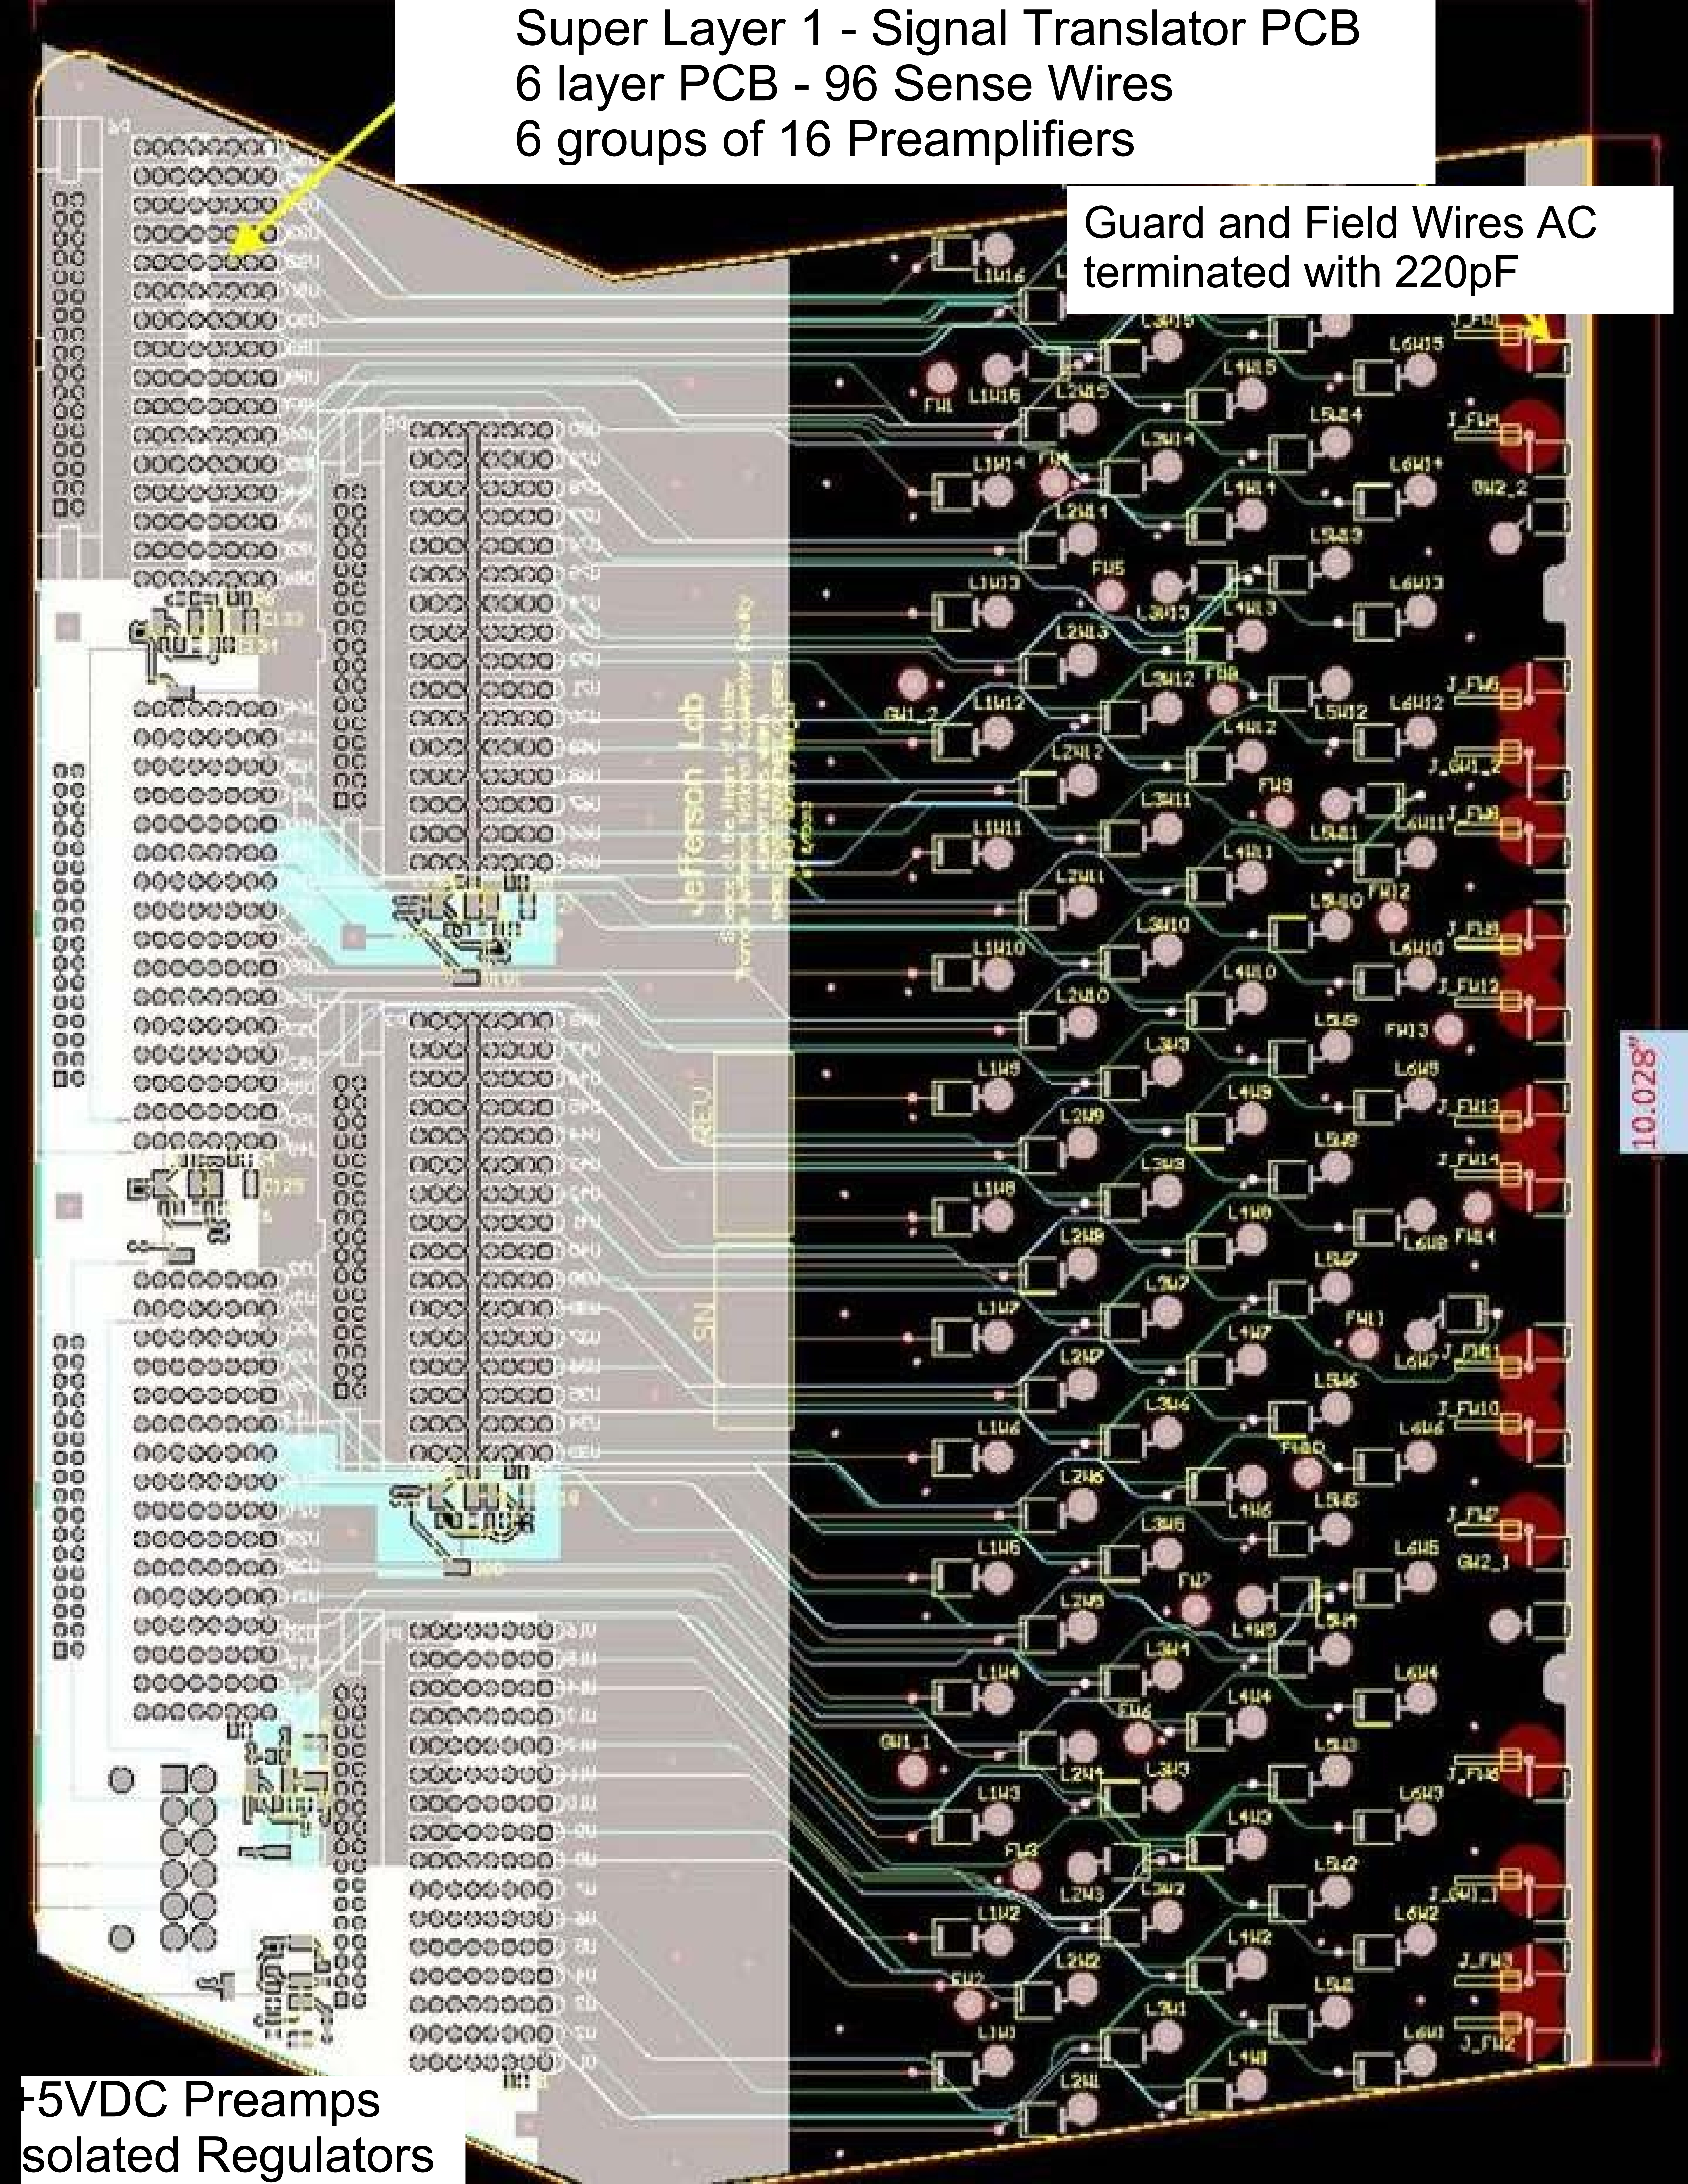
\includegraphics[width=0.7\textwidth,natwidth=610,natheight=642]{img/stb-layout.jpg}}}
\end{picture}
\caption{\small{Trace routing shown on one of the Region~1 STBs being
designed.}}
\label{stb-layout}
\end{figure}
%%%%%%%%%%%%%%%%%%%%%%%%%%%%%%%%%%%%%%%%%%%%%%%%%%%%%%%%%%%%%%%%%%%%%%%%%%%

\subsubsection{Single In-line Package (SIP) Preamplifiers}
The heart of the STB board is an individually packaged
single in-line package (SIP) preamplifer which was modified
from the design of the previous CLAS detectors and 
included an epoxy resin encapsulation.  
The encapsulation of the components prevents 
component corrosion in a somewhat humid environment (relative
humidities as high as 60\%).
These ``CP01'' pre-amplifiers provide the gain, dynamic range, rise time, low 
noise, and low power needed for the performance requirements.  The CP01 is
a transimpedance amplifier with a gain of 2 mV/$\mu$A and a rise-time
less than 10 ns.  Each SIP operates at 6V and draws about 13 mA.   

Fig.~\ref{CP01-description} shows the design and specifications of the
CP01 pre-amplifier.  See Ref.~\cite{fjb92} for the original design of
this SIP pre-amplifier.

%%%%%%%%%%%%%%%%%%%%%%%%%%%%%%%%%%%%%%%%%%%%%%%%%%%%%%%%%%%%%%%%%%%%%%%%%%%
\begin{figure}[htbp]
\vspace{8cm}
\begin{picture}(50,50)
\put(20,20)
{\hbox{\includegraphics[width=0.7\textwidth,natwidth=610,natheight=64]{img/CP01-description.jpg}}}
\end{picture}
\caption{\small{The CP01 pre-amplifier design and specifications.}}
\label{CP01-description}
\end{figure}
%%%%%%%%%%%%%%%%%%%%%%%%%%%%%%%%%%%%%%%%%%%%%%%%%%%%%%%%%%%%%%%%%%%%%%%%%%%

Each group of 16 pre-amplifier output signals was routed to a 17 pair connector.
Sixteen of the pairs are used as differential signal paths which are routed from the STB's to the 
drift chamber readout boards (DCRB) over individual cables consisting of 16 twisted pairs.  
We chose
twisted-pair readout because of its immunity to electronic noise.
The cables are round-jacketed with a 
0.025-in pitch so that the overall cable dimension is smaller than the 
standard 17-pair cable.  

\subsection{Off-Chamber Amplification, Time Digitization and Readout}

Our on-chamber 
pre-amplifiers send signals to the readout boards (DCRB) 
which provide another level of amplification, 
signal discrimination, adjustable threshold setting, time digitization
and readout. 

These DCRB's are based on FPGA technology, and in addition to
their primary function of amplification, discrimination, digitization
and readout, they are used in a simple ``cluster-finding'' algorithm
to find track segment candidates with a latency of only hundreds
of nanoseconds.

\subsubsection{Drift Chamber Readout Boards (DCRB)}

The DCRB is a 96 channel board that is a combination post-amplifier,
discriminator, time-to-digital converter (TDC) and also has a trigger
output path to provide track segment information for an online tracking trigger.
Fourteen such boards are housed in
a proprietary 9U, 160 mm depth, VXS form factor/crate.
The whole system consisted of 18 such crates, one for each drift chamber.

To perform its time digitization task, the DCRB utilizes on-board synchronization to
return the signal time relative to an input time signal from  a Trigger Distribution
Crate.
Its design and architecture
allows it to achieve the following performance metrics:
\begin{itemize}
\item DCRB Performance Metrics
\begin{itemize}
\item Amplification: variable gain from X10 to X30 eliminates saturation
\item Time Digitization: accuracy better than 1 ns; exceeds DC specifications
\item Whole Crate Time Synchronization: through backplane; eliminates cables
\item Event Buffer Size: 500,000 signals
\item VME Transfer Rate: 200 MB/sec
\item Maximum Trigger Rate: greater than 1 MHz
\item Dead-time: 32 ns
\item Scaler: 1 32 bit scaler per channel
\item Track Segment Finding: employs segment-hit dictionary in 32 ns bins
\item Track Segment Reporting: reports found segments to the next-level Track Finder
\end{itemize}
\end{itemize}

In addition to its primary functions of time digitization of DC signals and online
track-finding, the internal scaler functions allow the DCRB to be used in 
a stand-alone manner to efficiently monitor chamber operation during commissioning
and testing.

\subsection{Grounding Scheme}
We used a ``one-point'' grounding scheme.  The drift chambers themselves were insulated
from the torus magnet through use of an insulating portion of the link
mounting system.  The off-chamber readout boards (DCRB's) were likewise not grounded
to the chambers themselves though the use of non-grounded twisted-pair signals.
The low-voltage power supplies were floating, supplying a plus and minus line 
to the STB's.
The grounding point was at the High Voltage supply crates.  This was accomplished
by the use of two ground wires for every high-voltage 34-wire multi-cable.


% -------------------------------------------------
% electronics
% -------------------------------------------------

\section{Drift Chamber Utilities: Gas, Low Voltage and High Voltage Systems}

\subsection{Gas System: Mixing, Monitoring and Pressure Control}

The chambers operate on a gas mixture consisting of 90\% Argon and 10\% CO$_2$.
Using precision Mass-Flow Controllers (MFC), the gas is mixed and temporarily
stored in large-volume buffer tanks.  From these tanks it is delivered
to experimental hall B.  

Argon is supplied via boil-off from a large, permanent Dewar and CO2 is supplied 
via boil-off from several standard industry high-pressure Dewars. 2 identical mixing
systems are used to mix the gas to 90Ar/10CO2 by mass using regulators and MKS G250 
mass flow controllers (MFC).  The mixed gas is then stored at ~100psig in four large 
volume ASME pressure vessels, also called buffer tanks. This large volume smooths out 
any minor fluctuations in the Argon/CO2 ratio. To control the gas ratio, the thermal 
conductivity of the gas ratio is continually measured using Panametrics Thermal 
Conductivity Units (TCUs) and then matched to the thermal conductivity of a mixed 
gas calibration standard. Individual MFC flows are adjusted as needed if the gas mixture
ratio changes. The mixed gas is supplied to the hall via 3 identical gas delivery systems, 
one for each region. MFCs and pressure regulators set the gas flow and pressure from the 
buffer tanks to the supply manifolds in the hall. In the hall, flow control for each 
individual sector is set using rotameters located at the supply manifolds. The gas flows 
into each detector at the nose and exits out of the back-plate and into the exhaust 
manifolds. Since the gas volumes of R1 + R2 = gas volume of R3, R1 and R2 exhaust 
through the same manifold and R3 exhausts through its own manifold. The exhaust manifolds 
are connected to pressure relief systems. 

The Drift Chambers use thin, aluminized Mylar windows with a large surface area.  
Any over-pressure event could cause the windows to burst. Likewise, an under-pressure 
event could cause damage to the wires inside.  Due to the potential of catastrophic 
damage to the detectors in the case of an over-pressure or under-pressure event, 
passive relief systems (bubblers) are installed on each exhaust manifold. In an 
over-pressure situation (i.e. high differential pressure between the exhaust manifold 
and atmosphere), the gas in the detector is vented out until the differential pressure 
falls to a safe level. In an under-pressure situation (i.e. low differential pressure 
between the exhaust manifold and atmosphere), air is sucked into the exhaust manifold 
until the differential pressure increases to a safe level. Each of these high-flow 
differential pressure relief systems consist of 3 parts:  An oil filled over-pressure 
bubbler, an oil filled under-pressure bubbler, and an empty oil trap. The oil trap is 
connected to the exhaust manifold while the over and under pressure bubblers are 
connected directly to the oil trap. This prevents contaminating the exhaust manifolds
with oil. Additionally, each of the 3 parts contains baffles to remove oil droplets 
from the gas passing through the unit. 

Fig.~\ref{dc-gas-system} is a schematic of the gas delivery system 
and a snapshot 
of the control panel for monitoring the state of the system.

%%%%%%%%% Figure : dc gas system %%%%%%%%%%%%%%%%%%%%%%%%%%%%%%%%%%%%%%%%%%%%%%%
\begin{figure}[htbp]
\vspace{10cm}
\begin{picture}(50,50)
\put(-10,10)
{\hbox{\includegraphics[width=0.8\textwidth,natwidth=610,natheight=642]{img/dc-gas-system.png}}}
\end{picture}
\caption{\small{A schematic of the drift chamber gas system showing key control and
monitoring points.}}
\label{dc-gas-system}
\end{figure}
%%%%%%%%%%%%%%%%%%%%%%%%%%%%%%%%%%%%%%%%%%%%%%%%%%%%%%%%%%%%%%%%%%%%%%%%%%%%%%%


 
\subsection{Low Voltage System}
We reused tha low voltage power supplies that were used for {\tt CLAS}.  
These units are robust and manufactured by Hewlett Packard.  
The supplies are remotely programmable and monitored.   We 
isolated the low voltage from 
ground loops by using local voltage regulators on the pre-amplifier interface 
boards (STBs).  The segmentation of the low voltage distribution cables is 
based on 32 preamplifier channels per supply cable.  Each of these supply 
cables is fused with an appropriate type of fuse rated for over-current 
protection based on 32 pre-amplifier loads.  

We designed our low voltage system: supplies, fusing, cables and control
system to be as robust and maintenance-free as possible.  To minimize
the damage to the tracking system in the event of a failure such as
a shorted pre-amplifier, we built in fine segmentation with only
32 preamplifier channels per supply cable.  Each of these supply 
cables is fused with an appropriate type of fuse rated for over-current 
protection based on this load.
In the event of a short circuit which causes a fuse to blow,
a simple, external cable disconnect will reduce the size of the affected
area to 16 signal wires without the need to access the chambers.

The on-chamber pre-amplifiers require 6V and approximately 18A per chamber
(a total of 1344 pre-amps per chamber).
The low voltage power supplies are re-used from the original CLAS detector.  
These units are robust and manufactured by Hewlett Packard.  
The supplies are remotely programmable and monitored.   We 
isolated the low voltage from 
ground loops, using local voltage regulators on the pre-amplifier interface 
boards (STBs).  

Fig.~\ref{dc-lv-system} is a schematic of the low voltage
supply system and a snapshot 
of the control panel for monitoring the state of the system.
%%%%%%%%% Figure : dc low voltage system %%%%%%%%%%%%%%%%%%%%%%%%%%%%%%%%%%%%%%%%%%%%%%%
\begin{figure}[htbp]
\vspace{10cm}
\begin{picture}(50,50)
\put(-10,10)
{\hbox{\includegraphics[width=1.2\textwidth,natwidth=610,natheight=642]{img/dc-lv-system.png}}}
\end{picture}
\caption{\small{A schematic of the low voltage control and monitoring scheme.}}
\label{dc-lv-system}
\end{figure}
%%%%%%%%%%%%%%%%%%%%%%%%%%%%%%%%%%%%%%%%%%%%%%%%%%%%%%%%%%%%%%%%%%%%%%%%%%%%%%%

\subsection{High Voltage System}

As in the case of the low-voltage system, we designed our high voltage system: 
supplies, distribution boxes, cables and control system to be as robust and 
maintenance-free as possible.  
We re-used our CAEN 
system 527 high voltage supplies with somewhat finer segmentation than our 
previous system, consistent with our total channel count dropping from 34000 
to about 24000.
To minimize the damage to the tracking system in the event of a failure such as
a broken wire, we built in very fine segmentation.
Each individual high-voltage channel powers a variable-sized group of 
wires: a 48-wire group for wires in the small-angle region, a 96-wire group
in the middle-angle region and a 192-wire group at large angles.

In the event of a failure (e.g. a broken wire) which results in a trip
of a single HV channel, we can further reduce the size of the affected
area from the whole group (48, 96 or 192 wires) to a smaller grouping
of 48 wires by an external cable disconnect without the need to 
physically access the chambers themselves.

The high-voltage supply and distribution system consists of the following:
\begin{itemize}
\item a crate-based high voltage power supplies with 36 independent
high voltage channels for each drift chamber (1344 signal wires each).
Of these 36 channels, 16 supply positive high voltage to the sense
wires, 16 supply negative voltage to the field wires, and 4 supply
positive voltage to the guard wires
\item a series of two distribution boxes which distribute the high
voltage from the supplly channels on individual cables to groups
of wires, with the group size being 8 wires (for small angle wires)
to 16 (intermediate angles) to 32 (large angles). 
\item  on-chamber printed circuit boards which distribute high voltage
to all of the wires; these are the HVTB's
\end{itemize}



Fig.~\ref{dc-hv-system} is a schematic of the high voltage
supply system and a snapshot 
of the control panel for monitoring the state of the system.
%%%%%%%%% Figure : dc high voltage system %%%%%%%%%%%%%%%%%%%%%%%%%%%%%%%%%%%%%%%%%%%%%%%
\begin{figure}[htbp]
\vspace{10cm}
\begin{picture}(50,50)
\put(-10,10)
{\hbox{\includegraphics[width=1.\textwidth,natwidth=610,natheight=642]{img/dc-hv-system.png}}}
\end{picture}
\caption{\small{A schematic of the high voltage control and monitoring scheme, showing
the 1296 remotely controlled channels.}}
\label{dc-hv-system}
\end{figure}
%%%%%%%%%%%%%%%%%%%%%%%%%%%%%%%%%%%%%%%%%%%%%%%%%%%%%%%%%%%%%%%%%%%%%%%%%%%%%%%




% -------------------------------------------------
% gas, lv, hv systems
% -------------------------------------------------

\section{Pre-Commissioning and Installation}

In this section we describe the procedures that took
place after chamber stringing was complete in order to get the
chambers ready for installation and to install them 
in the experiment.

\subsection{Electronics Installation and Turn-on}
\label{electronics-installation}

After the chambers were strung and went through a mechanical quality
check to insure that all wires were intact and properly tensioned, we
installed the on-chamber electronics boards, using
the following procedures:
\begin{enumerate}
\item ``daisy-chained'' the field wire crimp pins so that a single
HV cable could power two rows of field wires (32 wires);
\item physically positioned the boards so that their plated through
holes aligned directly above the sense wire crimp pins, and attached
the boards to the chamber with screws;
\item electrically connected each sense wire crimp pin to each
plated through hole using a conductive elastomer tube that fit
over the crimp pin and also contacted the plated through hole on
its outer radius.
\end{enumerate}
A sketch of the process of attaching the circuit boards to the 
chambers is shown in Fig.~\ref{mounting-stb}.

%%%%%%%%%%%%%%%%%%%%%%%%%%%%%%%%%%%%%%%%%%%%%%%%%%%%%%%%%%%%%
\begin{figure}[htbp]
\vspace{5cm}
\begin{picture}(50,50)
\put(60,-5)
{\hbox{\includegraphics[width=0.3\textwidth,natwidth=610,natheight=642]{img/mounting-stb.png}}}
\end{picture}
\caption{\small{A sketch showing an on-chamber STB board being mounted.}}
\label{mounting-stb}
\end{figure}
%%%%%%%%%%%%%%%%%%%%%%%%%%%%%%%%%%%%%%%%%%%%%%%%%%%%%%%%%%%%%%

Now the chamber was ready for ``burn-in'' and ``pre-testing''.

\subsection{Burn-in and Pre-testing}

When drift chambers are first turned on, they typically draw fairly high
``dark'' currents, even at low voltages.  The standard procedure is to
slowly raise the high voltage, wait for a certain time period during
which the current subsides and raise the voltage again, and so on.
For our chambers, the typical time period was an hour and the typical
voltage step was 75~V.  For comparison, 90~V is approximately the 
``doubling voltage'' of
our chambers (the voltage step that increases the gain by a factor
of two).  The total time of ``burn-in'' for each chamber varied from one to three days.
Visual observation of good signals on an oscilloscope completed
the pre-testing.

\subsection{Installation and Survey}

The chambers are attached by ball-and-socket joints to rods that are attached
on the other end by ball-and-socket to the toroidal magnet frame.
After the initial installation, the chambers were moved to an approximate
working location.  Then, with the survey crew's information, the chamber location
was fine tuned by lengthening or shortening the rods with fine-pitch screw adjustments.
In this way the final chamber positioning was performed with sub-millimeter accuracies as
determined by the survey group's laser positioning system.

The installation of 18 chambers took months to accomplish and the survey crew's work
was hindered at times by obscured views of some of the fiducial marks on the 
chambers.  We checked and updated the survey information with a later 
``straight-track'' zero-field alignment run and analysis procedure (see Section~\ref{align}
for details of the alignment).
Although most of the alignment numbers were verified to sub-millimeter accuracy, there
were a few parameters that were off by as much as 2 mm.

Of particular note regarding the ``rod and ball-and-socket'' mounting scheme:
\begin{itemize}
\item by design, changing the length of any or all of the six links will
move the chamber in position and/or angle but will not apply stress to the
chamber,
\item once installed and surveyed, the chamber can be moved out to maintenance
position by changing only one of the link lengths,
\item this ``one link'' motion is reproducible to sub-millimeter accuracy, reducing the time
and manpower required for maintenace and repair.  In a matter of 8 hours, a chamber 
can be moved to ``maintenance position'', repaired, and moved back to installation
position without the need for a re-survey.  Fig.~\ref{maintenance-position} shows a single
chamber in maintenance position.
\end{itemize}

%%%%%%%%%%%% Figure : chamber in maintenance position  %%%%%%%%%%%%%%%%%%%%%%%%%%%
\begin{figure}[htbp]
\vspace{6.8cm}
\begin{picture}(50,50)
\put(-10,5)
{\hbox{\includegraphics[width=0.7\textwidth,natwidth=610,natheight=642]{img/maintenance_04.png}}}
\end{picture}
\caption{\small{A view of the 18 chambers mounted onto the torus magnet, with one
chamber moved out to maintenance position.}}
\label{maintenance-position}
\end{figure}
%%%%%%%%%%%%%%%%%%%%%%%%%%%%%%%%%%%%%%%%%%%%%%%%%%%%%%%%%%%%%%%


% -------------------------------------------------
% commissioning: ``burn-in and pre-testing'', installation and survey, lv, hv & gas hookup, signal connection
% turn-on, early failures and repair
% -------------------------------------------------

\section{Chamber Operation and Performance Monitoring}

\subsection{Choice of Gas}
\hskip 0.15in

The main requirements for the chamber gas were that it have reasonably low 
multiple scattering, allow for reasonable gas gains, have short collection 
times in order to reduce the random background expected from M{\o}ller 
electrons and target-generated X-rays, and be inexpensive because of the 
large volume of the chambers. Also, safety considerations motivate the use of
a non-flammable gas mixture.  Additional concerns about small gas 
leaks and the proximity of many photomultiplier tubes argued against helium 
mixtures.  Ultimately a 90$\%$ argon - 10$\%$ CO$_2$ mixture was employed 
for several reasons: the gas has a fairly high saturated drift velocity 
($>$ 5~cm/$\mu$s), and it has an operating voltage plateau of several hundred 
volts before breakdown occurs.  The 90$\%$/10$\%$ mixture 
provides good efficiency, adequate resolution, and reasonable collection times.




\subsection{Selecting the Proper Operating Voltage}
\hskip 0.15in
In this section we discuss our operating voltages and how it was selected.

First, we discuss how we divide the total voltage between our sense, field 
and guard wires in order to mimic a cell layout with an infinite number of
layers, to achieve a situation in which all wires, regardless of layer, have
the same gain.  Then we discuss our choice of the total sense to field
wire difference in voltage; including the resulting gas gain and efficiency.


\subsubsection{Dividing the Total Voltage between Sense, Field and Guard Wires}
As noted previously, we ran our chambers with a mixed voltage scheme:
positive high voltage on the sense wires, negative voltage on the
field wires and positive voltage on the guard wires.
This mixed-voltage scheme has a couple of advantgages over a scheme in
which the field wires, for example, are held at ground potential:
\begin{itemize}
\item fewer field lines run from the sense wire to the endplate which
is grounded.  This reduces the likelihood of producing a `Malter effect'
(Ref.~\cite{Malter}) in which an accidental source of cathode emission
(due to an insulating contaminant on the endplate, for example) causes
a self-sustaining discharge
\item the sense to ground potential and the field to ground potentials 
are smaller; decreasing surface electric fields on the on-chamber
circuit boards
\end{itemize}

In addition, by carefully selecting the values of the sense, field and
guard wire voltages we can create potential distributions which mimic
an infinite grid of cells, where the gain on any wire is the same as
any other, regardless of whether is the first, last or middle layer.

This optimum condition is reached when the sense voltage is twice the
field voltage (and opposite sign).  This is because we have twice as many
field wires as sense wires and all field lines which originate on a
field wire land on a sense wire.  

The guard wire voltage was then chosen so that the total charge on all wires is zero.  
If we have a nearby ground plane due to the metallized gas bag then it will
have no net effect on the nearby wire planes if there is no net flux of
electric field through the bag which is the case if the enclosed net charge
is zero.

So, the ratio of voltages from Sense to Field to Guard wires is 1 : -1/2 : 5/14.

\subsubsection{Operating Voltage, Gas Gain and Layer Efficiency}
The gas gain varies exponentially with the total sense to field wire voltage
difference, with a doubling voltage of about 100, 110 or 120V respectively, for
R1, R2 and R3.  During our Fall 2019 run, we ran with sense - field wire voltage
differences of 2100, 2325 and 2475 V, respectively for R1, R2 and R3

We calculate that our total gas gain is approximately 2.7~$10^4$, 3.7~$10^4$, and 4.4~$10^4$,  
respectively, for R1, R2 and R3.


References: `A study of electron drift velocity in Ar-CO2 and AR-CO2-CF4 gas
mixtures', NIM A340 (1994) p.485-490

CLAS-Note 2009-27 1Calculation of Drift Chamber Gas Gain' Mestayer


% -------------------------------------------------
%  operations and monitoring
% -------------------------------------------------

\section{Drift Chamber Calibration Procedures}
In this section, we discuss the calibration procedures to obtain the 
best possible spatial resolution for reconstructing the trajectory of
a forward-going charged particle.  We need to know three things to 
accurately reconstruct a trajectory: the location of the wires, the
distance of closest approach (DOCA) of the track to the wire and the
value of the magnetic field traversed.  These were determined by
\begin{itemize}
\item alignment procedures
\item time to distance calibration
\item magnetic field mapping and modelling
\end{itemize}.  We discuss all three after a brief overview of the track reconstruction.

\subsection{Track Reconstruction Overview}

\hskip 0.15 in
The reconstruction of charged-particle tracks is performed in several stages.  In 
the first stage, individual tracks are fit only to hit-wire positions in a 
procedure known as ``hit-based'' tracking.  Hit-based tracking proceeds
in the following steps:
\begin{itemize}
\item in each superlayer, ``clusters'' of hits which are consistent with
being part of a track are identified
\item a ``noise rejection algorithm'' is then applied to the clusters, 
with one of the more efficient algorithms being the removal of the
interior hits from horizontal ``strings'' of hits along a layer.
\item the resulting trimmed clusters are then fit to a straight-line hypothesis,
and those hits with acceptable residuals are kept and identified collectively
as a ``track segment''.  This fit uses the wire position as the assumed hit
position and is called ``hit-based tracking''.
\item because the ``hits'' in a track segment are 2-dimensional objects (we
do not know their location along the wire direction) a track segment is not
a line but a plane.  Thus pairs of segments in neighboring superlayers within
one chamber (with superlayers of +/- $6^\circ$ stereo angle) represent the
intersection of two planes; that is a line.  This line's coordinates 
are evaluated midway between the two superlayers, and is a 6-dimensional
object (x,y,z and 3 angles) which we call a ``cross''.
\item in the first pattern-recognition step to find a track candidate,
the positions of 3 crosses (1 each in R1, R2 and R3) are fit to a
parabolic functional form to give us a ``track candidate''.
\item the track candidate is the initial ``state vector'' of our
Kalman filter tracking program 
\end{itemize} 
The full track reconstruction procedure will be discussed in a separate paper.

Due to the comparatively small size of the drift cells and the large 
number of wire layers, the track momenta can already be reconstructed 
at the ``hit-based'' level with a 
resolution of 3$\%$ to 5$\%$.  Additional information on these tracks, derived
from the {\v C}erenkov, time-of-flight, and electromagnetic calorimeter 
detectors, allows for determination of the identities and speeds of the 
charged particles.  In the second stage of the analysis, flight-time 
information of the particles from the target to the outer scintillators is 
used to correct the measured drift times.  A pre-determined table is then used
to convert the corrected drift times to drift distances (see section~\ref{tdistcal} 
for details of the function). These corrected 
track positions in each drift cell are input data to our Kalman filter
fit to determine the final track parameters.  This is colloquially referred
to as ``time-based tracking''.

\subsection{Alignment Procedures}
\label{align}

\hskip 0.15in
As described in section~\ref{survey}, each of the 18 drift chambers was 
surveyed after installation into CLAS.  The survey procedures had sub-millimeter
accuracy, but we wanted an independent check of the chambers' positions.  For 
this reason, the survey values for the chamber geometry were viewed only as 
a reasonable starting point to be refined by comparisons with data.

To adjust the chamber geometry parameters to improve the tracking resolution,
``straight-track'' data with the torus magnetic field off were analyzed.  
Tracks were found and fitted with our standard track reconstruction package.
For various bins in the angle of the track, we measured the shifts of the
track residual means as a function of layer number. 
Before alignment, the data showed significant displacements of the means
from zero.  

Our procedure for aligment was straight-forward.  On a first pass through
the data we used misaligment parameters (shifts and rotations of individual
chambers) set to zero.  On subsequent passes, we deliberately misaligned
a particular chamber by a particular offset in position or angle and 
produced a second set of plots of residual mean vs. layer.  We ran 18 passes
through the data, adjusting all combinations of region (1, 2, 3) and
of offset type $\delta$x, $\delta$ y, $\delta$ z, $\theta$ x, 
$\theta$ y, $\theta$ z, one at
a time.  The offsets in $x, y$ and $z$ were 2 mm, and the angular rotations
were 0.2 degrees.  We called these ``unit distortions''.

We then subtracted the pass1 residual distribution from a pass``i'' distribution
to give a ``change of residual'' distribution caused by a given ``unit distortion''.
We then fit the observed residual distribution from the data to a weighted
sum of the 18 ``change of residual'' distributions.  In principle, we
could have had 18 free parameters, but in practice we had 12 free parameters:
 $\delta$ x, $\delta$ y, $\delta$ z, and $\theta$ y for each of the 3 chambers: R1, R2 and R3,
where $\theta y$ is a tilt of a chamber.  The yaw ($\theta x$) and roll ($\theta z$)
were not varied because they did not improve the fits.


The 
results of this procedure indicated that the best-fit position of the chambers 
along the three coordinate axes varied by up to several millimeters relative 
to the surveyed positions.  

\subsection{Time to Distance Calibration}
The drift chamber TDC's measure time.  This time is corrected for a number
of effects, and this corrected time is converted to a distance, DOCA, by 
a pre-calculated time to distance function.  In this subsection we 
explain the time corrections, the function used to calculate time as a 
function of DOCA and how we calibrate the parameters of this function.

\subsubsection{Time Corrections}
The drift time is the elapsed time between the time that the particle 
traversed the wire cell and the time that the released gas ions (electrons)
reached the sense wire.

The drift time is given by the following expression:
\begin{equation} 
\label{drift}
t_{drift} = t_{tdc} - t_{start} - t_{0} - t_{flight} - t_{prop} - t_{walk},
\end{equation}

\noindent
where $t_{TDC}$ is the raw time measured by the TDC, $t_{start}$ is the event start time, 
$t_0$ is the fixed-time (cable) delay for the wire, $t_{flight}$ is the 
flight time of the particle from the interaction vertex to the wire, $t_{prop}$ 
is the signal propagation time along the wire, and $t_{walk}$ is a time-walk 
correction made for short drift times due to different ionizations for slow 
and fast particles.  

With a trigger based on detecting an electron in the CLAS12 detector, the event start time is 
given by the time-of-flight counter time for the primary scattered electron 
corrected for the calculated flight time of this electron from the beam-target vertex.

Through the use of an appropriate function, the drift time determines the 
distance-of-closest-approach (DOCA) of the charged-particle track to the sense 
wire.  However, there remains an ambiguity regarding which side of the sense 
wire the track passed by.  This ``left-right ambiguity'' is resolved within 
the individual superlayers by comparing the $\chi^2$ values for the track fit 
for all different combinations of drift-distance signs.  After selection of 
the full set of drift-distance signs within each superlayer, a final fit 
results in improved track parameters.

\subsubsection{T0 Determination}
As indicated in eq(\ref{drift}), the fixed-time delays (mainly fixed cable delays) 
for each wire must be known in order to determine the drift times.   To determine
this t$_0$ value, we produced a histogram of the following quantity for all hits
used on tracks:$ ( t_{tdc} - t_{start} - t_{flight} - t_{prop} - t_{walk} )$.
This produced a characteristic plot of a drift chamber signal on a flat
background from out-of-time tracks.  Our 24,192 drift chamber signals are carried
on individually made multi-conductor cables which each carred 16 signals.  We thus
produced and analysed 24,192/16 = 1512 histograms to determine that many values of
t$_0$. We occasionally re-do this analysis whenever we have a new trigger condition
or new configuration of readout boards.


\subsubsection{Time-to-Distance Functional Parameterization}
\label{tdistcal}

\hskip 0.15in
Each hit on a track is characterized by two variables, the measured drift 
time from the sense wire and the distance-of-closest-approach (DOCA) to the 
sense wire resulting from the track fit.  
A best fit to the dependence of DOCA on time defines the 
drift-velocity function of the drift cells. However, several factors 
complicate this analysis. For example, the DOCAs obtained from the fitted 
tracks are biased quantities since an initial estimate of the drift-velocity 
function is used in the track determination.  Moreover, the drift cells are 
not circular, as the analysis implicitly assumes, but are hexagonal, leading 
to angle-dependent corrections.   The R2 chambers, in particular, are in a 
region of high and spatially varying magnetic field.  Finally, the different 
ionization densities of the tracks from particles with different velocities 
leads to substantial time-walk corrections for tracks near the wire.  Each of 
these points is briefly discussed in this section.


%%%%%%%%%%%%%%%%%%%%%% Figure : Garfield Picture %%%%%%%%%%%%%%%%%%%%%%%%%%
\begin{figure}[htpb]
\vspace{4.5cm} 
\special{psfile=garfield.eps hscale=49 vscale=49 hoffset=-15 voffset=-130}
\caption{\small{Plot of electric-field lines and equal-time isochrone contours
(100 ns interval) for a 90$\%$ argon - 10$\%$ CO$_2$ gas mixture for (a) an R3
drift cell where two rays are drawn highlighting two different track entrance 
angles of $\alpha$ = 0$^{\circ}$ and 30$^{\circ}$, and (b) an R2 cell that 
was assumed to be located within a uniform 1~T magnetic field along the z 
direction.}}
\label{garfield}
\end{figure}
%%%%%%%%%%%%%%%%%%%%%%%%%%%%%%%%%%%%%%%%%%%%%%%%%%%%%%%%%%%%%%%%%%%%%%%%%%%

Fig.~\ref{garfield} shows the isochrone contours and electric-field lines for 
a representative R3 and R2 cell.  Note that the contours are circular close 
to the wire but become hexagonal near the outer boundaries of the cell.  This 
illustrates the necessity of knowing the entry angle of the track in order to 
determine the drift distance to the sense wire from the measured drift time.

\subsubsection{Function Parameterization}
\label{funcpar} 

In the CLAS detector, the drift distance was parameterized and fit as a function
of drift time.~\cite{mdm95}.
For CLAS12, we have instead chosen to parameterize the time as a function of
distance.  This is a more natural description of the drift chamber signal
for several reasons:
\begin{itemize}
\item the maximum drift distance is given by geometry (the distance from
a sense wire to the nearest field wire) and so it is fixed
\item the drift velocity is a function of electric field strength, so the
point of minimum field is the point of minimum velocity (and thus the inflection point on the T vs X curve). 
This inflection point of the curve occurs at a
definite value of distance within the cell and not at a definite value of time.
\item the time walk due to finite ionization is
naturally parameterized as a function of distance and not as a function of time.
\item two of the major time corrections (time walk which is a function of the
particle $\beta$ and a time correction for wires in a magnetic field, $B$ which
scales like $B^2$) can simply be added to the nominal functional form.
\end{itemize}

A {\bf single functional form} is used to fill two tables: one of time indexed by discrete
values of distance for use in the simulation by GEMC and one of 
distance indexed by time for use by the track reconstruction code.


\subsection{Choice of Mathematical Forms for the Distance to Time Function}
We use a 4th order polynomial to model the distance to time relationship.

\begin{equation}
t(x) =  a x^4 + b x^3 + c x^2 + {1 \over v_0} x,
\end{equation}


By the use of simple calculus we convert the parameters a, b, c and d to equivalent parameters which have
a physically intuitive meaning (see next section).

\subsection{Physical Constraints on the Drift Velocity Function}

Inspection of  Fig.~\ref{garfield}a reveals that for tracks near the outer
edge of the cell, the first arriving ions follow the electric-field line from 
the field wire to the sense wire, independent of track entrance angle.  Their 
corresponding drift time is referred to as $t_{max}$ and is one of the fundamental
parameters of the function. 

A second constraint is that the velocity near the wire is the ``saturated drift
velocity'' for our gas mixture, 90$\%$ argon - 10$\%$ CO$_2$.  We call this parameter $V_0$.

Another constraint is imposed by the fact that there is a definite point in the
cell at which the electric field is a minimum.  This implies that this is the point
of minimum velocity and is thus an inflection point.  This occurs at a value
$r = (x/x_{max}) = 0.615$ and the drift velocity at this point is termed $V_{mid}$.

\subsubsection{Constraints on the Parameters for the Polynomial Form}
In this subsection, we present the algebra for the constraints on the parameters
(a, b, c and d) of the polynomial form.  Because there are four free parameters, we
have imposed four constraints.

Constraints on the function coefficients:
\begin{itemize}
\item  $t(x)$ must equal $t_{max}$ when $x = x_{max} $.
\item  the drift velocity near the sense wire ($x = 0$)
must equal the saturated value, $V_0$
\item the function has an inflection point (a
mininum in velocity) at the point in the cell with the lowest electric field
strength.  From the geometry of our cells, this occurs at a distance
of $ 0.615 \times x_{max}$.  Finally,
\item the velocity equals $V_{mid}$ at the inflection point.
\end{itemize}

To summarize, these are the four constraints on the distance to time functions:
\begin{enumerate}
\item $t(x = x_{max}) = t_{max}$
\item $dt / dx (x = 0) = 1 / V_0$
\item $d^2 t / dx^2 (\hat{x} = 0.615 ) = 0$   
\item $dt / dx (\hat{x} = 0.615 ) = 1/V_{mid}$  
\end{enumerate}

In this way we convert our original parameters, a, b, c and d to the physically meaningful
parameters $t_{max}, V_0, r, and V_{mid}$ where $r$ is the value 0.615 (the fractional distance
at which the inflection point occurs) which can in principle also be varied.


\subsection{Dependence of Distance to Time Function on Local Angle}
\noindent
The preceding was the derivation for the function of time as a function
of drift distance for tracks with a local angle, $\alpha = 30^0$.  
We now discuss the
functional dependence on varying local angle and on non-zero and varying
values of the B-field.

Please refer back to Fig.~\ref{garfield} which shows a 0 degree track and a 30 degree
track, both at maximum distance from the sense wire.  Note that they will give the
SAME TIME, Tmax, even though their distance-of-closest-approach differs by a factor
of cos(30deg).  If Dmax is the distance from sense to field wire (and the maximum
doca possible for a 30 deg. track), then Dmax times $\cos(30^\circ-\alpha)$ is the maximum
doca for a track with local angle, $\alpha$.  Call this distance, $Dmax_{\alpha}$.

\subsubsection{Local Angle Dependence of Polynomial Form}
We derived the function for time versus distance for a particular local angle, $\alpha$, by
assuming the same functional form as for $\alpha = 30$ but with a {\bf different coefficient, a}, which 
satisfies the constraint that  $F(dmax_{\alpha},\alpha)$ = $t_{max}$.

Using this constraint, we can solve for $a_{\alpha}$ in terms of the known coefficients $V_0, ~a, ~n$, and $m$,
yielding the following:
\begin{equation}
\label{aalphaequation}
a_{\alpha} = {{t_{max} - b dmax_{alpha}^3 - c dmax_{alpha}^2 - d dmax_{alpha}}\over{dmax_{alpha}^4}}
\end{equation}

Using this formula for $a_{\alpha}$ we can derive the time as a function of distance and local
angle, $\alpha$ as shown in Fig.~\ref{xvst}.  See, for instance, the upper-left sub-figure 
which shows the time as function of distance for 5 different angles between $0^{\circ}$ and 
$30^{\circ}$, equally spaced in $\cos \left(30^\circ-\alpha\right)$.  Note two things:
\begin{enumerate}
\item for each angle, $\alpha$, the time is $t_{max}$ at $dmax_{\alpha}$, and
\item the distances for a given time are linear in $\cos \left(30^\circ-\alpha\right)$.
\end{enumerate}

Thus, the general functional form for time as a function of distance and local angle, $\alpha$
is given by
\begin{equation}
\label{tfunctionofxandlocalangle}
t(x,\alpha) = a_{\alpha} x^4 + b x^3 + c x^2 + d x
\end{equation}




\subsection{Dependence of Distance to Time Function on Magnetic Field Strength}
Since the R2 chambers are located within the field region of the CLAS torus, the 
magnetic field affects the drift velocity as shown in 
Fig.~\ref{xvst}b.  In particular, the field rotates and shrinks the isochrones
as shown in Fig.~\ref{garfield}b.  These effects can be modeled by a 
modification to the effective entrance angle of the track and by an increase 
in the time at a particular DOCA.  Both of these corrections are assumed to depend only on the 
magnitude of the magnetic field, and not its direction, following a study 
described in Ref~\cite{MM-IEEE}.  

The rotation of the isochrones is parameterized as a shift in the effective
entrance angle.  
\begin{equation} 
\label{eq-bcorrn-to-ang}
\alpha_b = \alpha_0 + \alpha_c \cos^{-1}(1 - a B), 
\end{equation}

The correction term $\alpha_c$ is determined from a 
GARFIELD simulation to be:

\begin{equation} 
\label{eq-bang}
\alpha_c = \cos^{-1}(1 - a B), 
\end{equation}

\noindent
where $a$ is a constant equal to $0.02$ and $B$ is the magnetic field strength in Tesla and angular
units are degrees.

%%%%%%%%% Figure : TRKDOCA vs. Drift Time -- Angle and Field Dependence %%%%%%%%%%
\begin{figure}[htb]
\vspace{15.cm} 
\special{psfile=images/tvsx.eps hscale=80 vscale=80 hoffset=-20 voffset=-10}
\caption{\small{Scatterplot of the corrected drift time versus TRKDOCA for 
(upper-left) R1, showing curves for various local angles from 30$^{\circ}$
(righmost curve) to 0$^{\circ}$ (leftmost curve).  (Upper-right) for R2; 
additionally showing 3 bands for B-field magnitudes of 0, 1, 1.5 Tesla.
(Lower-left) for R3 with the inflection point identified.}}
\label{xvst}
\end{figure}
%%%%%%%%%%%%%%%%%%%%%%%%%%%%%%%%%%%%%%%%%%%%%%%%%%%%%%%%%%%%%%%%%%%%%%%%%%%%%%%


The maximum drift time used in the time-to-distance function was extracted 
directly from the data.  For R2 the maximum drift time was parameterized as:

\begin{equation} 
\label{eq-bmax}
t_{max}(B) = t_{max}(0) + b B^2,
\end{equation}

\noindent
where $b$ is a constant and $B$ is the magnetic field strength.

At any given local magnetic field point, the distance-to-time function 
includes an additional correction term $\delta t_B$ to describe 
the magnetic field dependence.  See this reference~\cite{qin96} for a related
parameterization of the change in the distance at a particular time due to a
B-field. 

\begin{equation}
\label{XTB}
t(\hat{x},\alpha,B) = t(\hat{x},\alpha-\alpha_c, B=0) +  \beta(\hat{x})*B^2.
\end{equation}

\noindent
In this expression, the first term is the time calculated assuming B=0, and the
second term is the time increase due to the B field.  For the R1 and R3 functions, no magnetic field 
dependence is included, as the chambers are located outside the torus 
cryostats in regions that are relatively field-free.


\section{Determining the Distance to Time Function Parameters}
We determine the experimental values of the function parameters by fitting
a histogram of $TRKDOCA$ vs. time.

\subsection{Method of Calibrating the Time-to-Distance Function}
\label{tdistcal}

Each hit on a track is characterized by two parameters, the measured drift 
time from the sense wire and the distance-of-closest-approach (TRKDOCA) to the 
sense wire.  A best fit to the dependence of time on TRKDOCA determines the
values of the parameters of the drift-velocity function. 

However, several factors 
complicate this analysis. For example, the TRKDOCAs obtained from the fitted 
tracks are biased quantities since an initial estimate of the drift-velocity 
function is used in the track determination.  Moreover, the drift cells and
the resulting isochrones are 
not circular, as the analysis implicitly assumes, but are hexagonal, leading 
to angle-dependent corrections.   The R2 chambers, in particular, are in a 
region of high and spatially varying magnetic field which affects the distance
versus time function.  Finally, the different 
ionization densities of the tracks from particles with different velocities 
leads to substantial time-walk corrections.  Each of 
these points is briefly discussed in the next section.
For these reasons, our fitting is an iterative process in which we calibrate,
re-do track fitting, re-calibrate, etc.  We usually converge in 1 or 2 iterations.

\section{Using the Distance to Time Function in Reconstruction}
The track reconstruction program needs to know the expected distance as a function
of time.  However, as explained in the previous paragraph, we will have calibrated and fitted
the observed time as a function of distance.  So, we need to NUMERICALLY INVERT the t=f(x)
function in order to fill a table of X (real number) as a function of the time index (integer).

\subsection{Filling the Time to Distance and Distance to Time Tables}
We calibrate the distance to time function by fitting the drift time versus
TRKDOCA at a particular local angle, alpha.  We write the independent parameters,
$V_0, V_{mid} amd T_{max}$ to the data-base.  At the beginning of a reconstruction program,
an $inversion program$ is run to numerical invert the function to produce a table
of distance indexed by time.


\subsection{How to Interpolate and Extrapolate in Local Angle}
Please refer back to Fig.~\ref{xvst} in order to understand the local-angle dependence
of distance versus time.  When the time is equal to $t_{max}$ the distance is equal to
the largest value for the local angle; that is, $dmax_{\alpha}$.  Also note that by
simple geometrical reasoning, $dmax_{\alpha} = dmax$  $cos(30-\alpha)$.
We assume that at times less than tmax and distances less than dmax, the calculated
distances still vary linearly as $cos(30-\alpha)$.  This angle dependence is built into
our functional form.

This means that we
\begin{itemize}
\item {\bf Fill} our time to distance tables for different local angles using the function, and
\item {\bf Interpolate} between time to distance tables for different local angles to obtain
the calculated distance at a particular local angle
\end{itemize}
For example if ``$X_0$'' is the distance (at a particular time) for a table filled for tracks with local angle of 0 degrees
and ``$X_{30}$'' is the corresponding quantity for a table of 30 degree tracks, then
\begin{equation} 
\label{eq-extrap30}
X(t,\alpha) = X_0 + (X_{30}-X_0) (cos(30-\alpha) - cos(30)) / (1. - cos(30))
\end{equation}





% -------------------------------------------------
%  tracking, calibration and simulation
% -------------------------------------------------

\section{Drift Chamber Tracking System Performance}

In this section, we describe the tracking system performance: the ability to operate at high luminosity,
the efficiency at reconstructing charge particle tracks, and the spatial resolution of such tracks.

\subsection{Operation at High Luminosity}

In order to satisfy the statistical requirements of the experimental program, an important design
goal for CLAS12 is the ability to make routine measurements with electron beam luminosities up to
10$^{35}$~cm$^{-2}$s$^{-1}$.  The luminosity limit in CLAS12 is 
set by the large flux of M{\o}ller electrons and low-energy photons 
produced from the targets by the multi-GeV incident electron beam.  This 
constraint is severe for the drift chambers since they are close to the 
target. 

Particularly for the R1 chambers, the large flux of particles limits the luminosity in several ways.
First, the chambers must be able to operate with an acceptably low trip rate.
Second, the accidental occupancy in the chambers should be on the order
of 5\% or less in order to keep the track-finding inefficiencies at a moderate 
level.  See the accompanying article on track reconstruction (\cite{recon-nim})
for a quantitative discussion of this effect.  Third, the effects of sustained high 
luminosities can be unfavorable for long chamber lifetimes.  Aging correlates 
directly with the currents generated in the chambers.
However, our choice of an argon-CO$_2$ gas mixture and strict control of
materials in contact with the gas should provide a long chamber lifetime.
For the previous CLAS chambers, we used the same gas mixture and ran at a
similar gain and similar currents, and the chambers lasted more than 10 years 
with no indication of aging.  We expect the present
chambers to perform well for at least 10 years.

\subsection{Tracking Inefficiency: Intrinsic, Malfunction-Related, and Background-Related}

The probability of reconstructing a track due to a charged particle within our fiducial volume
is referred to as the ``tracking efficiency''. The tracking inefficiency has three root causes:

\begin{enumerate}
\item {\bf intrinsic layer inefficiency}: the failure to record
a hit for a track crossing a layer, when all wires and electronics
are operating properly;
\item {\bf malfunction-related inefficiency}: loss of hits and sometimes
whole track segments because of equipment malfunctions;
\item {\bf background-related inefficiency}: out-of-time background
can interfere with the segment-finding algorithms when a background-related
track segment lies ``on top'' of a real, in-time, segment.
\end{enumerate}

\subsubsection{Simulation of Inefficiencies}

In our generation and reconstruction of simulated events, we estimate the size of
the three types of inefficiency in the following manner:

\begin{enumerate}
\item {\bf simulation of intrinsic layer inefficiency}: this is a random process
and, as such, it is handled at event generation time by our Monte Carlo simulation
program GEMC~\cite{sim-nim}.  For each superlayer (1-6), we have defined a DOCA-dependent
layer inefficiency function, as determined from the data.  At hit-generation
time in GEMC a random number (between 0 and 1) is generated, and if it is
smaller than the layer inefficiency function, the hit is not digitized.
\item {\bf simulation of malfunction-related inefficiency}: the GEMC Monte
Carlo hits are generated as if there are no malfunctions of the wires.
During the Monte Carlo reconstruction, however, a status table for each
hit wire is queried and if the wire is in the ``bad status'' list, that
hit is not used in the tracking.  The malfunction-related inefficiency  is small.  
At the time of publication, roughly $0.5\%$ of our wires are not operating properly.  
\item {\bf simulation of background-related inefficiency}: rather than try
to simulate out-of-time background due to all physics processes, we merge
``random-trigger'' events with events from low-luminosity runs and compare the
efficiency of these merged events with that from un-merged low-luminosity events.
This ratio is considered to be a measure of the background-related inefficiency.
\end{enumerate}

We will not further discuss the {\bf malfunction-related inefficiency} or
the {\bf background-related inefficiency} further in this article.  See
our companion article on track reconstruction for more details~\cite{recon-nim}.

Here we present our results on measuring the {\bf intrinsic layer inefficiency}.

\subsubsection{Intrinsic Layer Inefficiency}

The layer efficiency is the probability that a
good hit is recorded in a wire layer through which the track has passed, based on 
the evidence from all other layers in the superlayer.  This is called the 
``excluded-layer method''.  The layer efficiency is a measure of the intrinsic drift 
cell efficiency for the particular choice of gas mixture, high-voltage set point, and 
discriminator level.  


The single layer inefficiency is not uniform across the drift cell.  It is higher near the sense wire and also
near the outer edge of the cell.  A track passing close to a sense wire leaves many ions in the cell, but the
ion arrival times are stretched out from near-zero to the maximum drift time $Tmax$.  The result is that
the preamplifier's output signal has a low voltage amplitude but persists for a long time.  So, even though
the collected charge is large the voltage put out by our transimpedance preamplifiers may not be large
enough to exceed the voltage discriminator threshold of the DCRB. For the case of tracks near the outer
edge of the cell (so-called `corner-clippers') they leave a very small number of ions in the cell and
thus have a small signal.

Fig.~\ref{dc-inefficiency-vs-doca} shows that a large contribution to the inefficiency comes 
from tracks that pass close to the sense wire.  These tracks give rise to signals 
that have low pulse height and long duration, and thus may escape detection.
We fit this observed DOCA-dependent inefficiency to a functional form that is
used in our GEMC Monte Carlo hit digitization routine to randomly throw out
this percentage of hits.

%%%%%%%%%%%%%%%%%%%%%%%%%%%%%%%%%%%%%%%%%%%%%%%%%%%%%%%%%%%%%%%%%
\begin{figure}[htbp]
\vspace{5.7cm}
\begin{picture}(50,50)
\put(70,0)
{\hbox{\includegraphics[width=0.6\textwidth,natwidth=610,natheight=642]{img/dc-inefficiency-vs-doca.png}}}
\end{picture}
\caption{\small{The observed ``layer efficiency'' as a function of DOCA.  Hits from tracks
that pass close to or far from the sense wire have the hits spread out in time, and the resulting
voltage pulse from the preamplifiers may fail to cross the discriminator threshold, resulting
in a ``lost hit''.}}
\label{dc-inefficiency-vs-doca}
\end{figure}
%%%%%%%%%%%%%%%%%%%%%%%%%%%%%%%%%%%%%%%%%%%%%%%%%%%%%%%%%%%%%%%%%%%

\subsection{Drift Chamber Spatial Resolution}

The single-wire resolution is the RMS spread of the difference 
between the fitted TRKDOCA of the track and the value of DOCA as calculated from the 
time of the hit.  The variance of this residual distribution 
is the quadratic sum of the single-wire resolution and the track position uncertainty.  
This variance over-estimates the single-wire resolution.
Since there are six layers per superlayer,
this amounts to a $10 - 15\%$ over-estimate.

Fig.~\ref{resolution-vs-doca} shows the width of the track-hit residual distribution plotted versus
TRKDOCA for each of the different chamber regions.  The single-wire resolution worsens near the 
wire and also at the outer edge of the cell.  This arises due to finite cluster sizes 
due to the Poisson distribution of ion-pair production along the path of the primary ion 
near the sense wire along with time walk effects and the divergent nature of the electric
field lines near the field wire.  

%%%%%%%%%%%%%%%%%%%%%%%%%%%%%%%%%%%%%%%%%%%%%%%%%%%%%%%%%%%%%%%%%
\begin{figure}[hbtp]
\vspace{7.3cm}
\begin{picture}(50,50)
\put(50,-10)
{\hbox{\includegraphics[width=0.85\textwidth,natwidth=610,natheight=642]{img/resolution-vs-doca.png}}}
\end{picture}
\caption{\small{The hit resolution plotted versus TRKDOCA for R1, R2, and R3 (top, middle, bottom),
    respectively.}}
\label{resolution-vs-doca}
\end{figure}
%%%%%%%%%%%%%%%%%%%%%%%%%%%%%%%%%%%%%%%%%%%%%%%%%%%%%%%%%%%%%%%%%%%

A more quantitative look at the resolution as a function of DOCA is given in Fig.~\ref{resid-vs-doca},
for data from all six R3 drift chambers.
The upper sub-figure is a plot the 2-D distribution of the fit residual (TRKDOCA - DOCA) vs. TRKDOCA.
We did a Gaussian slice-fit in the x-coordinate (TRKDOCA) and plotted the resulting sigma from
each fit versus TRKDOCA in the lower sub-figure.
The average single-wire resolution in the middle 
portion of the cell is about 250~$\mu$m, with a whole cell resolution of about 400~$\mu$m. 
Looking at similar fits for all of the chambers, we conclude that the whole-cell 
average is about 400~$\mu$m for R1, R2, and R3, respectively.  

%%%%%%%%%%%%%%%%%%%%%%%%%%%%%%%%%%%%%%%%%%%%%%%%%%%%%%%%%%%%%%%%%
\begin{figure}[htbp]
\vspace{8cm}
\begin{picture}(50,50)
\put(40,-5)
{\hbox{\includegraphics[width=.8\textwidth,natwidth=610,natheight=642]{img/resid-vs-doca.png}}}
\end{picture}
\caption{\small{Upper figure: a plot of residual vs. TRKDOCA.  Lower figure: a plot of the Gaussian sigma of the
upper plot (from a slice-fit) vs. TRKDOCA.}}
\label{resid-vs-doca}
\end{figure}
%%%%%%%%%%%%%%%%%%%%%%%%%%%%%%%%%%%%%%%%%%%%%%%%%%%%%%%%%%%%%%%%%%%

\subsection{Conclusions}

The toroidal geometry of the CLAS spectrometer necessitated a particle-tracking 
system of unconventional design.  Design challenges and solutions include the following:

\noindent
- The necessity to conceal inactive areas of the drift chambers within the
shadow regions of the torus cryostat resulted in very thin endplates and low-profile
wire connection schemes and on-board preamplifiers.

\noindent
- The toroidal shape of the magnet and the desire to have measurements before, within, 
and after the high-field region, resulted in the design of a ``rod and ball'' mounting scheme
that minimizes dead areas and facilitates maintenance.

\noindent
- The fabrication of chambers that support large static wire tensions, but have thin 
endplates necessitated three endplate designs: aluminum stiffened with steel bars (R1),
Stesalit an epoxy-G10 composite) stiffened with steel bars (R2), and carbon fiber plates filled with foam and reinforced
with carbon-fiber posts on the entrance side and a carbon-foam-carbon composite plate on the exit side (R3). 

\noindent
-The need for precise tracking in a system with non-saturated drift velocity 
(necessitated by the requirements of large drift distances, non-flammable gas mixtures, 
and low-gain operation) resulted in a semi-automated calibration and monitoring software 
package.

\vskip 10pt
The CLAS12 drift chamber system has been in routine operation since spring, 2017. 
The system has reached its design goals of high-luminosity operations in beam
(1$\times$10$^{35}$~cm$^{-2}$s$^{-1}$) in a high-flux electromagnetic reaction
environment, with very good track reconstruction efficiency over a large range of angles and 
magnetic fields~\ref{recon-nim}.  
The percentage of malfunctioning wires, due to high voltage problems, signal
connector issues, etc., is presently ~0.5\%.
The single-wire efficiency is greater than $98\%$ and the
single-wire resolution is about 400~$\mu$m averaged over all drift distances and
all 18 chambers, with each chamber showing a characteristic 250~$\mu$m resolution 
in the cell center.

\vskip 10 pt

{\large{\bf Acknowledgments}}

\vskip 10pt

The authors wish to thank the crews of wire stringers and technicians who 
participated during the chamber construction at the Idaho State University,
Old Dominion University, and Jefferson Laboratory, as well as the support of 
the technicians involved with installation of the detectors into CLAS12.  The
authors also thank Dr. Simon Taylor for his careful reading of the draft.  This
work was supported in part by DOE contract DE-AC05-84ER40150, DOE grants 
DE-FG02-87ER40315, DE-FG05-94ER40859, DE-FG02-96ER40960, DE-FG02-96ER40980, 
and NSF grant NSF-PHY-9412479.






% -------------------------------------------------
%  track resolution and efficiency
% -------------------------------------------------

\begin{thebibliography}{99}

\bibitem{}

\bibitem{dcnim} M.D. Mestayer {\it et al.}, Nucl. Inst. and Methods A {\bf 449}, (2000) 81-111.

\bibitem{clasnim} B.A. Mecking {\it et al.}, Nucl. Inst. and Methods A {\bf 503}, (2003) 513-553.

\bibitem{cathode-emission} S.B. Christo and M.D. Mestayer, ``Minimizing Cathode Emission in Drift 
Chambers'', CLAS-Note 92-016, (1992).

\bibitem{patent} U.S. Patent 8,863,568 ``Apparatus and procedure to characterize the surface quality 
of conductors by measuring the rate of cathode emission as a function of surface electric field 
strength'', Mac Mestayer, Steve Christo, Mark Taylor.

\bibitem{kadyk}
J.A. Kadyk, Nucl. Inst. and Methods A {\bf 300}, 436 (1991).

\bibitem{nasa} W. Campbell and J. Scialdone, ``Outgassing Data for 
Selecting Spacecraft Materials'', NASA internal report RP-1124 Rev. 3 (1993).

\bibitem{sbc} S.B. Christo, ``Considerations for Crimping the
CLAS Drift Chamber Wires'', CLAS-Note 89-021, (1989).

\bibitem{stesalit} S. Bernreuther {\it et al.}, Nucl. Inst. and Methods A {\bf 367}, 
96 (1995); W.L. Imhof {\it et al.}, Space Science Reviews {\bf 71}, 305 (1995).

\bibitem{stesalitaging} R. Bouclier {\it et al.}, Nucl. Inst. and Methods A {\bf 350}, 
464 (1994).

\bibitem{malter} L. Malter, Phys. Rev. 50, 48 - 58 (1936)

\bibitem{fjb92}
F.J. Barbosa, ``A Preamp for the CLAS DC'', CLAS-Note 92-003, (1992).

\bibitem{mdm92} M.D. Mestayer, ``Choosing the Correct 
Combination of Sense, Field, and Guard Wire Voltage'', CLAS-Note 
92-005, (1992).


\bibitem{mdm95}
M.D. Mestayer {\it et al.}, Nucl. Inst. and Methods A {\bf 367}, 316 (1995).

\bibitem{MM-IEEE} M.D. Mestayer {\it et al.}, IEEE Transactions on Nuclear 
Science {\bf 39} No. 4, 690 (1992).

\bibitem{qin96} L.M. Qin {\it et al.}, ``Performance of a Region II Drift Chamber Prototype and Region II Drift Chamber Tracking'', CLAS-Note 96-018, (1996).

\bibitem{torus-ieee} Probir K. Ghoshal {\it et al.} IEEE Transaction on Applied Superconductivity, Vol. 29, No. 4, June 2019.

\bibitem{magmapping}
J. Newton {\it et al.} ``Measuring and Modelling the CLAS12 Torus Magnetic Field'', CLAS-Note (to be written)






\bibitem{cdr}
CEBAF Hall B Conceptual Design Report (1990).




\bibitem{cathode}
S.B. Christo and M.D. Mestayer, ``Minimizing Cathode Emission in Drift 
Chambers'', CLAS-Note 92-016, (1992).















\bibitem{dscnim}
D.S. Carman {\it et al.}, Nucl. Inst. and Methods A {\bf 419}, 315 (1998).

\bibitem{ereport}
R.A. Schumacher and R. Magahiz, ``The Region 1 Drift Chamber 
Endplates: Procurement History and Inspection Results'', CLAS-Note 
94-018, (1994).

\bibitem{ansys}
S.J. Bianculli, Master's Thesis, University of Pittsburgh (1993).

\bibitem{rat}
R.A. Thompson {\it et al.},``Issues in Stringing the CEBAF Large 
Acceptance Spectrometer Region 1 Drift Chamber", CLAS-Note 96-019, 
(1996).

\bibitem{r2nim} L.M. Qin {\it et al.}, Nucl. Inst. and Methods A {\bf 411}, 265 (1998).

\bibitem{chew89} M. Chew {\it et al.}, ``Investigations into Wire Sag in the
CLAS Drift Chambers'', CLAS-Notes 89-016, 89-017, (1989).

\bibitem{roth}
S.A. Roth and R.A. Schumacher, Nucl. Inst. and Methods A {\bf 369}, 215 (1996).

\bibitem{r1survcn}
R.A. Schumacher, ``Region One Drift Chamber Analysis of Survey Data'',
CLAS-Note 98-001, (1998).



\bibitem{mfv96}
M.F. Vineyard, T.J. Carroll, and M.N. Lack, in Proceedings of the 1995 International
Conference on Accelerator and Large Experimental Physics Control Systems, 
edited by M. Crowley-Milling, P. Lucas, and P. Schoessow (Fermilab Report 
CONF-96/069), W-PO-37 (1996).

\bibitem{GARFIELD}
GARFIELD has been developed at the University of Mainz by R. Veenhof and
revised by M. Guckes and K. Peters.  See HELIOS-note 154, (1986).

\bibitem{carman2}
D.S. Carman, ``CLAS Region I Prototype Detector", CLAS-Note 96-022,
(1996); The measured gain corresponds to that within a 200 ns time window.

\bibitem{carman}
D.S. Carman {\it et al.}, ``Hall B Test Run : Drift Chamber Studies", CLAS-Note
97-001, (1997).

`A study of electron drift velocity in Ar-CO2 and AR-CO2-CF4 gas
mixtures', NIM A340 (1994) p.485-490

CLAS-Note 2009-27 ``Calculation of Drift Chamber Gas Gain'' Mestayer


\end{thebibliography}


% -------------------------------------------------

\end{document}

